\documentclass[10pt,conference]{IEEEtran}
%\IEEEoverridecommandlockouts
% The preceding line is only needed to identify funding in the first footnote. If that is unneeded, please comment it out.
\usepackage{cite}
\usepackage{amssymb,amsfonts}
%amsmath,
\usepackage{mathtools}

\usepackage{algorithmic}
\usepackage{graphicx}
\usepackage{textcomp}
\usepackage{xcolor}
\usepackage{bussproofs}

\usepackage{pgf}
\usepackage{tikz}
\usepackage[utf8]{inputenc}
\usetikzlibrary{arrows,automata}
\usetikzlibrary{positioning}

\usepackage{etoolbox}
\usepackage{holtexbasic,url,amsmath,environ}
\renewcommand{\HOLTokenTurnstile}{\ensuremath{\vdash\!\!}}
\renewcommand{\HOLinline}[1]{\ensuremath{#1}}
\renewcommand{\HOLKeyword}[1]{\mathsf{#1}}
\renewcommand{\HOLConst}[1]{{\textsf{\upshape #1}}}
\renewcommand{\HOLTyOp}[1]{\textsf{\itshape #1}}
\renewcommand{\HOLSymConst}[1]{\HOLConst{#1}}
\renewcommand{\HOLTokenBar}{\ensuremath{\mathtt{|}}}

\newtheorem{theorem}{Theorem}
\newtheorem{corollary}{Corollary}
\newtheorem{definition}{Definition}
\newtheorem{remark}{Remark}
\newtheorem{example}{Example}
\newtheorem{conjecture}{Desideratum}
\ifdef{\dpspecial}{
%% tmp by Dirk
\newcommand{\HOLtm}[1]{\texttt{#1}}
\newcommand{\HOLty}[1]{\texttt{#1}}
\newcommand{\HOLthm}[2][]{\texttt{#2}}
\newcommand{\n}{\\n}
}{}
\NewEnviron{holthmenv}{\[\begin{array}[t]{l}\BODY\end{array}\]\ignorespacesafterend}
\newcommand{\TODO}[1]{{\bf TODO:} #1}

\def\BibTeX{{\rm B\kern-.05em{\sc i\kern-.025em b}\kern-.08em
    T\kern-.1667em\lower.7ex\hbox{E}\kern-.125emX}}
\begin{document}

\title{Modular Synthesis of Verified Verifiers of Computation with STV Algorithms}
%*\\
%{\footnotesize \textsuperscript{*}Note: Sub-titles are not captured in Xplore and
%should not be used}
%\thanks{Identify applicable funding agency here. If none, delete this.}


\author{\IEEEauthorblockN{Milad K. Ghale}
\IEEEauthorblockA{\textit{The Australian National University} \\
%\textit{name of organization (of Aff.)}\\
Canberra, Australia \\
milad.ketabghale@anu.edu.au}
\and
\IEEEauthorblockN{Dirk Pattinson}
\IEEEauthorblockA{\textit{The Australian National University} \\
%\textit{name of organization (of Aff.)}\\
Canberra, Australia \\
dirk.pattinson@anu.edu.au}
\and
\IEEEauthorblockN{Michael Norrish}
\IEEEauthorblockA{\textit{Data61, CSIRO, and ANU} \\
%\textit{Data61, CSIRO, and ANU}\\
Canberra, Australia \\
Michael.Norrish@data61.csiro.au}
%\and
%\IEEEauthorblockN{4\textsuperscript{th} Given Name Surname}
%\IEEEauthorblockA{\textit{dept. name of organization (of Aff.)} \\
%\textit{name of organization (of Aff.)}\\
%City, Country \\
%email address}
%\and
%\IEEEauthorblockN{5\textsuperscript{th} Given Name Surname}
%\IEEEauthorblockA{\textit{dept. name of organization (of Aff.)} \\
%\textit{name of organization (of Aff.)}\\
%City, Country \\
%email address}
%\and
%\IEEEauthorblockN{6\textsuperscript{th} Given Name Surname}
%\IEEEauthorblockA{\textit{dept. name of organization (of Aff.)} \\
%\textit{name of organization (of Aff.)}\\
%City, Country \\
%email address}
}

\maketitle
\begin{abstract}
\end{abstract}

\begin{IEEEkeywords}

\end{IEEEkeywords}
\section{Introduction}\label{sec:intro}
%\setlength{\abovedisplayskip}{0.5em}
%\setlength{\belowdisplayskip}{0.5em}
\section{Evidences}
\label{sec:DataEv}
%\section{The Generic STV Algorithm}
%\label{sec:GenSTV}
%%%%We shall initially clarify what the problem is that we are trying to address. 
%Then we proceed to elaborate on our approach and detail about the solution. 
%%%%%  To this end assume an arbitrary scheme $\mathcal{A}$ belongs to the STV family.The question is given any imp $\mathcal{P}$ is any implementation of $\mathcal{A}$ where the source code of $\mathcal{P}$ is  secret. 
%The question is how can one verify  $\mathcal{P}$ implements $\mathcal{A}$ correctly so that computation carried out by $\mathcal{P}$ is trustworthy?
%%%%The question is how can one verify that each execution of $\mathcal{P}$ correctly computes the end result in accordance with instructions in $\mathcal{A}$?

%Although full static verification is the most desirable answer to prove correctness, it is not practically possible here due to inaccessibility of source code. But even if the source were available it would not be feasible to carry such a task  because verifying every single implementation for any arbitrary STV algorithm is a Herculean significantly resource consuming agenda. Besides, any small change in implementation of an algorithm may render the whole  static verification of the implementation useless to the point that the process need to be redone from the scratch.   
We are motivated to 
%engineer a trustworthy practical  framework to answer the 
tackle the following problem. How can one verify that any execution of any implementation $\mathcal{P}$ whose source code is secret of an arbitrary  known STV algorithm $\mathcal{A}$ correctly computes the end result according to  $\mathcal{A}$?  



To begin 
%with addressing the problem, 
assume $\mathcal{P}$ is an implementation of an algorithm $\mathcal{A}$. We reasonably demand each execution of $\mathcal{P}$ on a given input $x$ consisting of ballots recorded in the election to output the winners $y$ and evidence $\omega$ as claim  for correctness of the execution.
%of the election for an input $x$ consisting of election votes recorded. Given the situation, what is also sensible to ask and easy to be produce, is to make $\mathcal{P}$  also output an evidence $\omega$ of correctness of $y$. 
 Having evidence available for each execution of $\mathcal{P}$ facilitates checking correctness of the computation carried out \emph{independently} of the (source code of) $\mathcal{P}$. Therefore the original problem boils down to how one can verify the evidence of any \emph{instance of computation} with any algorithm $\mathcal{A}$.


%New questions emerge from the above problem reformulation.  
The evidence as such must be enough informative to provide transparency of tallying and also allow  voters, or at least a large pool of scrutineers, to verify for themselves that the tally is authentically processed as per instructions of the counting scheme  so that winners truly reflect will of the voters. 
%Note that evidences are produced by various instances of computation with many STV algorithms which differ from each other in their exact counting mechanism.  
Therefore the questions becomes what information is enough 
%for satisfying transparency and independent verifiability of tallying 
for establishing transparency and verifiability of tallying  and what data structure for recording the information in evidence we should choose.

%%As mentioned above, STV algorithms vary in their precise algorithmic content.  On the other hand, we aim at producing verified verifiers of evidences of these divergent algorithms through a modular process that allows us to synthesise evidence verifiers of different schemes  throughout a uniformly replicable procedure.  Hence another challenge is what generic mechanism can we craft to produce verified verifiers that validate evidences of an STV algorithm distinctively and yet be able to employ that same process for creating another verifier for a different scheme while minimising the effort in synthesising it.  



\subsection{Characterisation of Evidence}
%%%Through thorough analysis of various STV schemes, we come to identify a common underlying data and algorithmic structure existing in the family. We abstract this structure as a finite state machine and call it the \emph{generic STV}\cite{}. Upon each execution on a given input $x$, the machine outputs a value $y$ and an \emph{evidence} $\omega$ which is the trace of all states that the machine visits from an initial machine state where $x$ is registered to the final state where $y$ is obtained.   
%%%%%Concrete STV algorithms are therefore realised as instantiations into the machine. Each of the instantiations  also produce an evidence for any instance of computation carried out. 
%%%%%%%Our objective here is to independently scrutinise process of counting under any STV schemes similar to physical scrutineers who observe tallying to attest its authenticity.  Having an evidence of computation at hand, we are then able to validate or reject the instance of computation carried out by checking if all of the transitions taken to terminate at the final state where the winners are declared are correct.  
A comprehensive analysis of different STV algorithms reveals existence of a common underlying abstract data type among STV algorithms as follows. 
%Each STV scheme operates on the following data.
\begin{itemize}
\item Some ballots to deal with (assuming) recorded as cast by voters. Each ballot is a pair consisting of a list expressing the preference of a voter and a fractional transfer value,
\item a quota which is the least amount of votes needed to attract in order to be elected, 
\item some candidates competing in the election, 
\item some number of vacancies for which candidates compete,
\item \emph{discrete states of computation} which encapsulate necessary  pieces of information needed to transparently know how the tallying has progressed from the beginning to the end and to be able to independently verify its correctness provided access to the information is granted. 
\end{itemize}
There are two kinds of discrete states of computation. Some of them are final states where tallying has reached a halting state by finding the winners of the election. The other consist of non-final ones where bits and pieces of data are manipulated according to counting mechanism of the STV scheme used, to eventually obtain an end result. Each non-final state comprises seven pieces of data: 
\begin{itemize}
 \item\textbf{uncounted ballots} which await being counted,
 \item\textbf{tally} for holding information about the amount of votes that each candidate has hitherto attracted %up to this state of computation,
 \item\textbf{pile} to know the ballots allocated to each candidate, 
 \item\textbf{backlog of elected} candidates who have exceeded the quota and their surplus votes awaits being transferred,
 \item\textbf{backlog of eliminated} ones whose votes awaits transfer,
 \item\textbf{elected candidates} who are the already elected ones whose surplus votes must be transferred,
 \item\textbf{continuing candidates} still continuing in the election. 
 \end{itemize}
%Data recorded in the final and non-final states as specified above   record all of the information needed and sufficient to know for independently validating a counting instance. 

The non-final and final states specified above provide us with all information one needs. We therefore find a perfect characterisation for evidence. 
\begin{definition}\label{formalEv}
Suppose an STV algorithm $\mathcal{A}$ is given and $Q$, $s$ and $C$ are respectively the quota, number of vacancies and competing candidates in an electon whose counting algorithm is $\mathcal{A}$ . Also assume  $y$ is the output of an execution of $\mathcal{A}$ on an input $x$. By evidence $\hat{\omega}$ for the execution  we mean the quadruple $(Q,s,C,\Omega)$, where $\Omega$ is the chronological sequence of all states of this instance of computation visited from the initial state where $x$ is input to the final state where $y$ is output.   
\end{definition}
%\begin{definition}[Evidence]
%An evidence $\hat{\omega}$ for an instance of computation with an algorithm $\mathcal{A}$ is a trace of data whose abstract representation matches with some formal evidence. 
%\end{definition}
%Definition asserts the abstract data type whose values mathematically represent a state of computation. A sequence of these mathematical states formally represent an evidence. In other words, an evidence is a trace of data whose abstract characterisation is a member of the mathematical construct given in Definition. 
%\begin{definition}
%Assume $\mathit{Ballot}$, $\mathit{Tally}$, $\mathit{Pile}$ are respectively sets of ballots, tallies, and pile of ballots. Also assume $\mathcal{C}$ is the set of all of competing candidates in  an election. Then the set of final states equals to the set of all subsets of $C$, namely $2^{C}$, and the set of non-final states are 
%\begin{small}
%\begin{center}
%$\mathit{Ballot}\times\mathit{Tally}\times\mathit{Pile}\times (2^{C}\times 2^{C})\times 2^{C}\times 2^{C}$
%\end{center}
%\end{small}
%where the fourth component represents backlog of elected and removed and the last two ones are respectively for elected and continuing candidates. 
%\end{definition}
\section{The Generic STV  Machine}
\label{sec:Machine}
\setlength{\abovedisplayskip}{0.5em}
\setlength{\belowdisplayskip}{0.5em}
We have already discussed an abstract data type whose values  formally represent evidence. However we do not yet possess an operational semantics for manipulating data to validate evidence.   On one hand, the semantics must be flexible enough to accommodate variations existing in the counting mechanism of STV algorithms so that we can produce verifiers  specifically operating for validation of evidence output by their associated scheme. On the other hand it must facilitate designing and developing the framework modularly while offering automation of synthesising process of verifiers.
%in such a way that we achieve a desirable degree of modularity and automation of  the process of synthesising different verifiers.
%evidence verifiers for various STV algorithms.


%STV algorithms vary in their precise algorithmic content.  On the other hand, we aim at producing verified verifiers of evidences of these divergent algorithms through a modular process that allows us to synthesise evidence verifiers of different schemes  throughout a uniformly replicable procedure.  Hence another challenge is what generic mechanism can we craft to produce verified verifiers that validate evidences of an STV algorithm distinctively and yet be able to employ that same process for creating another verifier for a different scheme while minimising the effort in synthesising it. 

%\subsection{STV Algorithms Analysis II}

In a secondary examination of the STV family, we also identify a general algorithmic mechanism for performing computation on evidence, which realises the \emph{commonalities} among the family members. This generic method comprises seven general actions~(Figure~\ref{GenSteps}) corresponding to actions that tally officers take when counting votes.
\begin{figure} 
 \begin{itemize}
\item\textbf{count} for counting the uncounted ballots,
\item\textbf{elect} for electing all or some of the electable candidates, 
\item\textbf{transfer-elected} for distributing surplus votes of elected, %candidates, 
\item\textbf{eliminate} to exclude one or some candidates, 
\item\textbf{transfer-removed} to distribute votes of   the eliminated, %candidates, 
\item\textbf{elected-win} for terminating tallying whenever the vacancies are filled or there is no continuing candidate left, 
\item\textbf{hopeful-win} for terminating tallying whenever  the number of already elected and continuing candidates collectively does not exceed the initial vacancies. 
\end{itemize}
\caption{Generic STV Counting Steps}
\label{GenSteps}
\end{figure}
Each action is constituted of  pre-conditions on when and how the action comes into effect, and post-conditions dictating what effect applying the action brings about by describing the new state to which computation proceeds. In fact, these conditions are the formal counterparts of the legal clauses in the textual specification of the counting scheme which tell tally officers how to proceed with tallying, and they are common between all flavours of STV. 

For example a constant pre-condition for applying elimination  asserts that there must be no uncounted ballot left and another one declares that no candidate should be electable at the current state of counting. A post-condition of elimination is that once a candidate is excluded from counting, the list of continuing candidates is updated accordingly so that the excluded candidate no longer received votes. Conjunctions of such declarations comprise what an action is and what an application of that action means.


The underlying abstract data type and the universal algorithmic pattern found in STV characterise components of a finite state machine which we call \emph{generic STV}~(Definition\ref{STVMachine}). The set of machine states consist of the discrete states of computation $\mathcal{S}$ mentioned earlier. The seven generic actions form the transition labels $\mathcal{T}$ of the machine. Last, the everywhere present pre- and post-conditions which define (content of)  the actions, make a small-step operational semantics for the machine.
% \begin{remark} 
Note that the states of computation recorded in all possible  evidence now become identical with machine states.
%states of the generic STV. 
%\end{remark}

\begin{definition}[The generic STV machine]\label{STVMachine}
Let $\mathcal{S}$  and $\mathcal{T}$
be respectively the set of machine states and transition labels.  Also assume for $t\in\mathcal{T}$, $S_{t}$ $=$ $\bigwedge_{\atop{i\leq j_{t}}} \psi_{i}$ where  $\psi_{i}$ is the formal specification (in higher-order logic) of a pre- or post-condition of $t$. Then \emph{generic STV} is the triple $M = \langle \mathcal{S}, \mathcal{T}, (S_t)_{t \in \mathcal{T}} \rangle$. 
%where $S_t$ is the sanity check condition  for  transition $t \in \mathcal{T}$.  An \emph{instance} of $M$  is a tuple $I = \langle \mathcal{T}, (R_t)_{t \in \mathcal{T}} \rangle$, where for each $t \in \mathcal{T}$, $R_t \subseteq \mathcal{S} \times \mathcal{S}$ is a rule that satisfies the sanity check condition $S_t$. 
\end{definition}
There are nonetheless variations in STV algorithms  which we  recognise  by separate \emph{instantiations} into the machine.  
\subsection{Instantiations of the Machine with Specific STV schemes}
Differences exist between counting algorithms of STV schemes.  
 For example in the STV used for electing the upper house representatives of the Victoria state of Australia (Victoria STV), distributing votes of an eliminated candidate occurs step by step in order of the magnitude of the fractional values that those votes carry.  Consequently, a pre-condition for applying the action is to first assure that upon each instance of applying transfer-removed action (a) exactly those votes which have the same fractional value are transferred and (b) the transfer happens according to the magnitude order. In contrast, for example, the STV used in the lower house elections of Tasmania state of Australia (Tasmania STV) does not have such pre-condition simply because votes of an eliminated candidate are transferred in a single application of transfer-removed. There are also variations in post-conditions. For example transfer-elect of the ACT STV used in the lower house elections of the ACT state of Australia requires distributing only the last parcel of surplus votes received by an elected candidate. But Victoria STV specifies transferring all surplus votes of an elected candidate.  


We formally realise variations of STV algorithms by instantiation~(Definition\ref{STVInst}) of the generic machine. Recall that the semantics of the machine is formed by conjunctions of formally specified universally appearing pre and post-conditions in STV algorithms. An instantiation of the machine with an STV algorithm $\mathcal{A}$ happens by enriching the generic semantics by adding formal specifications of the legal clauses that are specific to $\mathcal{A}$. We hence come to define an operational semantics functioning in accordance with instructions of $\mathcal{A}$. 
\begin{definition}[Instantiation of the Machine]\label{STVInst}
Assume the generic machine $M = \langle \mathcal{S}, \mathcal{T}, (S_t)_{t \in \mathcal{T}} \rangle$ as in Definition~\ref{STVMachine}. An instantiation $\hat{\mathcal{A}}$ for an STV algorithm $\mathcal{A}$ into the generic STV machine $M$ is a triple $\langle \mathcal{S}, \mathcal{T}, (S'_t)_{t \in \mathcal{T}} \rangle$, where for each $t\in\mathcal{T}$, $S'_{t}$ $=$ $S_{t}\wedge\bigwedge_{\atop{i\leq j'_{t}}} \phi_{i}$. Each $\phi_{i}$ is the formal specification of a pre- or post-condition specific to $\mathcal{A}$.   
\end{definition}

The operational semantics of each instantiation allows  to perform operations such as validation on evidence. Definition~\ref{verifier} lays down what verifying an evidence amount to. Informally speaking, to check if  evidence is valid one simply needs to inspect if transitions  between each two consecutive states of computation appearing in the evidence occur by a legitimate application of a counting action of the scheme used.

\begin{definition}[verifier]\label{verifier}
Assume $\hat{\mathcal{A}}= \langle \mathcal{S}, \mathcal{T}, (S'_t)_{t \in \mathcal{T}} \rangle$ is an instantiation of the STV algorithm $\mathcal{A}$. A verifier for instances of computation with $\mathcal{A}$ is a function $\hat{\mathcal{V}}$ mapping from $\mathbb{Q}\times\mathbb{N}\times 2^{C}\times$ \textsf{List}$(\mathcal{S})$ to $\{0,1\}$ such that for any evidence $\hat{\omega} = (Q,s,C,\Omega)$ where $\Omega=\langle\Omega_{1},\dots,\Omega_{n}\rangle$, $\hat{\mathcal{V}}(\hat{\omega}) = 1$ if and only if the following holds:\\
$\forall i\in\{1,\dots,n-1\}.$ 
%\hspace*{0.2cm}$\forall \Omega_{i-1}$ $\Omega_{i}\in\mathcal{S}.$
%$\exists \Omega_{1}$ $\Omega_{2}\in$ \textsf{List} $(\mathcal{S}).$ $\Omega = \Omega_{1} + [\Omega_{i-1};\Omega_{i}] + \Omega_{2}$  
$\exists t\in\mathcal{T}.$  $(\Omega_{i-1},\Omega_{i})\in t$ $\wedge~\vdash\mathcal{S}'_{t}[\Omega_{i-1},\Omega_{i}]$\\ 
where $\mathbb{Q}$ and $\mathbb{N}$ respectively represent the set of rational and natural numbers, $2^{C}$ is the set of all subsets of $C$, and \textsf{List}$(S)$ is the set of all possible lists of machine states. $\Omega_{i-1}$ is a pre-state and $\Omega_{i}$ is a post-state visited in the execution. The last line means that pre- and post-conditions  of applying $t$ to move from $\Omega_{i-1}$ to $\Omega_{i}$  are logically true. 
\end{definition} 

We shall next provide an example to concretely illustrate a piece of evidence and exemplify how STV schemes work. 

%In the rest of the paper we discuss technicalities of design  and development of the framework  for modular synthesis of formally verified verifiers. 
%However we first provide an example of an evidence to concretely illustrate them and exemplify how counting with an STV scheme works. 

%Equipped with the suitable semantics, we can define what verifiers of evidences are and how they validate data provided in evidences. Assume a formal evidence $\omega$ $=$ $(Q,s,C,\Omega)$ for an instance of computation with an STV scheme $\mathcal{A}$ is given. A formal verifier $\mathcal{V}$ for $\mathcal{A}$ is a function that recursively checks if any two consecutive machine states $s_{1}$ and $s_{2}$ in $\Omega$ each two consecutive machine states in the sequence $\Omega$  
%%%%%%%%%%%%%%%%%%%%%%%%%%%%%%%%%%%%%%%%%%%%%
%%%%%%%%%%%%%%%%%%%%%%%%%%%%%%%%%%%%%%%%%%%
%%%%%%%%%%%%%%%%%%%%%%%%%%%%%%%%%%%%%%%%%%%%%%%%
%\section{A Concrete Evidence of a Real STV Algorithm}
% To provide an sensible example of what a real STV algorithm resembles and how a concrete instance of an evidence is, we first present the algorithm used in ACT state of Australia for electing the representatives of the lower house. Then we given an example of an execution of the algorithm on a fictional election. 
%\subsection{STV Algorithm of ACT State Australia}
%\label{subsec:ana}
%We continue the quest by first analysing the whole STV family. Through this examination we obtain insight into what  data evidences should encapsulate and what structure is suitable for organising the data.
%Moreover, we realise a generic method which lays the foundation for  modular design and implementation of the framework for synthesising verifiers.



%The protocol dictates how to perform computations in two sets of instructions. It first gives the general steps to be taken whenever appropriate and then details conditions required for those steps to occur.
%\begin{description}
%\item[Step~1.] 

%%\noindent\textbf{Step~1.} Count the first preference votes for each candidate.
%\item[Step~2.]

%\noindent\textbf{Step~2.} calculate the quota according to the following formula;\\
%(total number of valid votes / (number of vacancies) + 1) + 1
%\item[Step~3.] 

%%%\noindent\textbf{Step~3.} Any candidate with votes equal to or greater than the quota is declared elected. If all vacancies have been filled, then the election finishes. Otherwise, if any candidate have more votes than the quota then go to step~4, and if no candidate has exceeded the quota then go to step~5.
%\begin{itemize}
%\item[$\bullet$] if all vacancies have been filled, then the election finishes.
%\item[$\bullet$] if all vacancies have not been filled, does any candidate have more votes than the quota?
%\begin{itemize}
%\item if yes, then go to step~4
%\item if not then go to step~5
%\end{itemize}
%\end{itemize}
%\item[Step~4.]

%%%\noindent\textbf{Step~4.} Distribute the successful candidate's surplus votes to continuing candidates according to the further preferences shown on the ballot papers by those voters. 

%\item[Step~5.]
%%%%\noindent\textbf{Step~5.} If there are more continuing candidates than there are vacancies remaining unfilled, exclude the candidate with the fewest votes and distribute this candidate's votes to continuing candidates according to the further preferences shown by those voters. Calculate each continuing candidate's new total votes then go back to step~3. If the number of continuing candidates is equal to the number of vacancies remaining, all of those candidates are declared elected and the election is completed.
%\end{description}

%The protocol further elaborates on the constraints for and effects of application of counting, electing, transferring, or eliminating candidates;
%\begin{description}
%\item[Counting the first preferences.] 

%%%%\noindent\textbf{Counting first preferences.}   Count the number of first preference 
%(or number \lq\lq~1\rq\rq) votes for each candidate.  
%After all the formal first preference votes are counted, the quota can be calculated.  
%%%Any candidate who has votes equal to or greater than the quota is now elected.
%\item[Transferring surplus votes from elected candidates.]
 %If a candidate receives a total number of votes equal to or greater than the quota, the candidate is elected. If an elected candidate has received an exact quota of votes, all of those votes are set aside and not counted further. 

%%%%\noindent\textbf{Transferring surplus of elected.}  The value of the surplus votes gained by an elected candidate is passed on to other candidates according to the preferences indicated on ballot papers by the voters. If a candidate has received more than a quota 
%of first preference votes, all the ballot papers received by the candidate are distributed at a reduced value called a fractional transfer value. If a candidate has received more votes than the quota following a transfer of votes from another elected candidate or from an excluded candidate, only that 
%%%%all the ballots that the candidate received at the last count of preferences which resulted in a surplus of votes,  called \emph{last parcel} of ballots, are distributed to continuing candidates at a fractional transfer value.
%After the surplus votes from an elected candidate have been distributed, the total number of votes which each candidate has received is recalculated. 
%%%%Any other candidates that have votes equal to or greater than the quota are elected. If vacancies remain, the surplus votes of any newly elected candidate are now  distributed one by one.
%\item[The fractional transfer value.] 
%\noindent\textbf{Fractional transfer value.}
%%%%The fractional transfer value is calculated using the following formula:\\
%%%(number of surplus votes) / (total number of ballot papers with further preferences shown)
%\item[Excluded candidates.] 

%%%\noindent\textbf{Elimination.} If vacancies remain to be filled after all surplus votes from elected candidates have been distributed, the process of excluding the lowest-scoring candidate begins. 
%\begin{itemize} 
%%%% The candidate with the smallest number of votes is "excluded" and his or her ballot papers are distributed to continuing candidates according to the preferences shown by the voters.
%%%% Ballots from excluded candidates are distributed at the value at which they were received by the excluded candidate. %Ballot papers received by the candidate as first preference votes have a value of \lq\lq~1\rq\rq~, while ballot papers received following the distribution of a surplus will have a fractional transfer value. 
%This will vary depending on the group of surplus votes from which they were received. 
%%%At each stage after ballot papers have been distributed from an excluded candidate, the total votes received by each continuing candidate are recalculated.
% to determine whether any candidate has received votes equal to or greater than the quota. 
%\end{itemize}

%%%%%%%%The process of distributing surplus votes from elected candidates and excluding the candidate with the fewest votes continues until all vacancies are filled.
%\end{description}
 \subsection{An Example of a Concrete Piece of Evidence}
\label{subsec:InstEv}
Figure~\ref{EvInst} depicts evidence of a small election whose counting algorithm is the ACT STV 
with three candidates $a$, $b$ and $c$, and initially recorded ballots containing
$b_1=([a,c],1/1)$, $b_2=([a,b,c],1/1)$, $b_3=([a,c,b],1/1)$,
$b_4=([b,a],1/1)$, $b_5=([c,b,a],1/1)$.  The first component of each ballot is a preference-ordered list of candidates, and the second is the fractional transfer value (initially set to $1/1$). The evidence consists of a \emph{header} that specifies the quota (computed according to the ACT STV instructions), the number of vacancies, and the list of competing candidates. 
The fourth line is the election result, and the remainder of the evidence are non-final states visited to compute this
outcome. Each non-final state shows uncounted ballots, tallies of candidates, piles of votes attracted, backlog of the elected, backlog of the eliminated, list of elected candidates, and list of continuing candidates. 

First preferences for each candidate are computed, and ballots counted in favour of particular candidates are placed onto that candidate’s pile. Here, $a$ is the first preference on $b_{1}$, $b_{2}$, and $b_{3}$, and $b$ receives $b_{4}$, and $c$ receives $b_{5}$ . Tallies are updated so that tally of $a$ becomes 3, and $b$
and $c$ each reach $1/1$. As $a$ exceeds the quota, he is elected and the fractional value of his surplus is updated according to the ACT scheme. Then $a$'s surplus is transferred to continuing candidates $b$ and $c$ and votes are counted according to next preferences shown on $a$'s surplus votes. Candidate $b$ and $c$ each attracts one vote. However  neither of them reaches to the quota. Therefore the weakest one $b$ is eliminated. As the number of elected and continuing candidates does not exceed the initial vacancies, the election terminates by declaring $a$ and $c$ winners.
\begin{small} 
\begin{figure}[b]
\begin{tabular}{c@{\hspace{2cm}}c} 
\AxiomC{\tiny 8/3} \noLine

\UnaryInfC{\tiny 2} \noLine \UnaryInfC{\tiny $[a,b,c]$} \noLine

\UnaryInfC{\scriptsize [a,c]} \LeftLabel{\tiny hwin}

\UnaryInfC{\tiny [$b_4$,([a,b,c],1/9)]]; a\{3/1\} b\{10/9\} c\{11/9\}; a\{[]\} b\{[]\}
c\{[[$b_{5}$,([c],1/9),([c,b],1/9),([c],1/9)]]\}; []; [a]; [c]}

\LeftLabel{\tiny elim} \UnaryInfC{\tiny []; a\{3/1\} b\{10/9\}
c\{11/9\}, a\{[]\} b\{[[$b_4$],[([a,b,c],1/9)]]\}
c\{[[$b_5$],[([a,c],1/9),([a,c,b],1/9)]]\}; []; [a]; [b,c]}

\LeftLabel{\tiny count} \UnaryInfC{\tiny
[([a,c],1/9),([a,b,c],1/9),([a,c,b],1/9)]; a\{3/1\}
b\{1/1\} c\{1/1\}; a\{[]\} b\{[[$b_4$]]\} c\{[[$b_5$]]\}; []; [a]; [b,c]}

\LeftLabel{\tiny tr-elect} \UnaryInfC{\tiny []; a\{3/1\} b\{1/1\}
 c\{1/1\}; a\{[[([a,c],1/9),([a,b,c],1/9),([a,c,b],1/9)]]\}
b\{[[$b_4$]]\} c\{[[$b_5$]]\}; [a]; [a]; [b,c]} \LeftLabel{\tiny elect}

\UnaryInfC{\tiny []; a\{3/1\} b\{1/1\} c\{1/1\}; a\{[[$b_1$,$b_2$,$b_3$]]\}
b\{[[$b_4$]]\} c\{[[$b_5$]]\}; []; []; [a,b,c]} \LeftLabel{\tiny count}

\UnaryInfC{\tiny ba; a\{0/1\} b\{0/1\} c\{0/1\}; a[] b[] c[]; []; [];
[a,b,c]} \DisplayProof \end{tabular} \caption{An example of  Evidence} \label{EvInst} \end{figure} \end{small}

\section{The Framework Architecture}\label{sec:Arc} 
We progress through three macro-level phases to develop the framework. For the first phase we use HOL4 to formally specify, implement and verify the generic STV, its instantiations, verifiers, and every auxiliary assertions needed for these ends. The second step relies on the verified proof translation tool of CakeML to provably correctly translate implementations of the first phase into equivalent CakeML implementations. The last phase uses the ecosystem of CakeML and its verified compiler to generate machine executable evidence verifiers.   


Figure~\ref{PicArc} is a simplified schematic illustration of the framework modules and their dependencies. We explain the purpose of each and then describe how they collectively function.

\paragraph*{\textbf{Auxiliary}} The module contains specification, implementation and verification of the generic STV. It consists of subdivisions for formal specification of the machine and its components, implementation of functions  meant to be the computational counterparts of the specifications and verification of the implementations by proving that they logically satisfy their respective specifications. Moreover we include specification, implementation and verification of helper assertions which appear in many well-known STV schemes here so that Auxiliary also serves as a comprehensive library for STV. 
\paragraph*{\textbf{Instantiations}}
  Instantiations of the generic STV happen in separate modules which we have schematically shown only two, namely   \textbf{STV}$_{1}$ and \textbf{STV}$_{2}$. An instantiation module \textbf{STV}$_{i}$ for an algorithm $\mathcal{A}$ consists of a subdivision for specification $\hat{\mathcal{A}}_{spec}$ of  the scheme and another one its implementation $\hat{\mathcal{A}}_{dec}$. 
\paragraph*{\textbf{Proofs}} We prove that for an algorithm $\mathcal{A}$ in the above modules,  $\hat{\mathcal{A}}_{dec}$ is logically equivalent to $\hat{\mathcal{A}}_{spec}$. We automate proofs so that they work for various instantiations. 
%Therefore all it would take for users is to instantiate the machine with their favoured STV scheme, if it was missing in our framework.
\paragraph*{\textbf{Verifier}} This module formally realises  the notion of verifier in Definition~\ref{verifier}. However, it is developed in a way that automatically operates  regardless of which STV algorithm is instantiated into the machine. It has three subdivisions. A  specification $\hat{\mathcal{V}}_{spec}$ defining what a verifier is, the implementation $\hat{\mathcal{V}}_{dec}$ and proofs of equivalence of $\hat{\mathcal{V}}_{spec}$ and $\hat{\mathcal{V}}_{dec}$.
\paragraph*{\textbf{Translation}} We translate each implementation $\hat{f}_{imp}$ in HOL4 to a proven  equivalent implementation $f_{\tau}$ in CakeML's environment by using the verified proof translator of CakeML. For example, an implementation  $\hat{\mathcal{A}}_{imp}$ of a scheme $\mathcal{A}$ and its   verifier $\hat{\mathcal{V}}_{imp}$ are  respectively translated into $\mathcal{A}_{\tau}$  and $\mathcal{V}_{\tau}$. 
\paragraph*{\textbf{DeepSpec}} 
For any translated verifier $\mathcal{V}_{\tau}$ and the translated evidence parser $\mathcal{P}_{\tau}$, we obtain logically equivalent deep CakeML embeddings  $\mathcal{V}^{*}$ and $\mathcal{P}^{*}$, respectively. We then use them to establish end-to-end desired properties, based on CakeML's I/O model, about the interaction of the executable verifier with its hosting operating system. 
%These properties rely on CakeML's modelling of I/O mechanisms.   
%For example, we prove that whenever an evidence does not accord with the grammar, we receive an appropriate message about the mismatch.    

\tikzset{
    state/.style={
           rectangle,
           rounded corners,
           draw=black, 
           minimum height=2em,
           inner sep=2pt,
           text centered,
           },
}
\begin{figure}[t]
\centering
%\framebox[\columnwidth]{
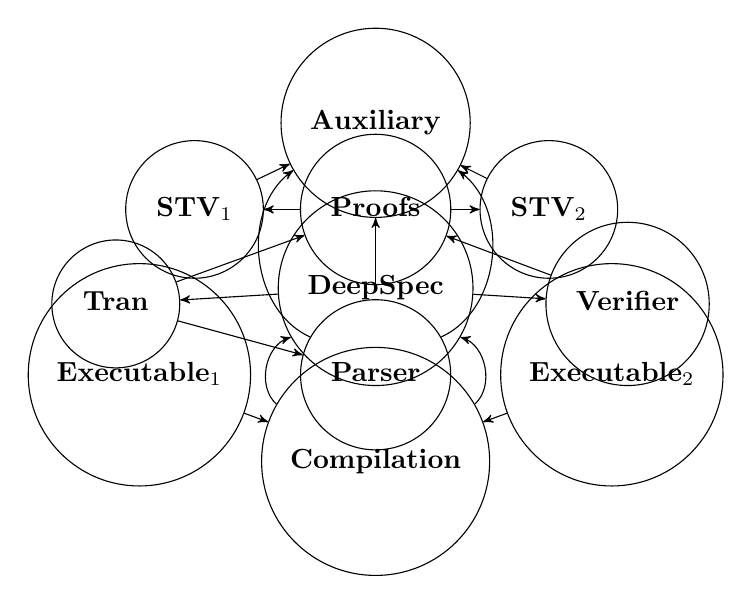
\begin{tikzpicture}[->,>=stealth']

 % Position of PARAM 
 % Use previously defined 'state' as layout (see above)
 % use tabular for content to get columns/rows
 % parbox to limit width of the listing
 \node[state] (Aux) 
 {\begin{tabular}{l}
  \textbf{Auxiliary}
 \end{tabular}};
 
  % STATE STVONE
 \node[state,
  below of=Aux,
  %yshift = -2cm,
  node distance=1.1cm,
  anchor=center] (proof) 
 {%
 \begin{tabular}{l}
  \textbf{Proofs}
 \end{tabular}
 }; 
  
   % STATE PARAM
 \node[state,
  left of= proof,
  xshift = -1.3cm,
  %node distance=1.5cm,
  anchor=center] (STV1) 
 {%
 \begin{tabular}{l}
  \textbf{STV$_{1}$}
 \end{tabular}
 }; 
 
  % STATE STVTWO
 \node[state,
  right of= proof,
  xshift = 1.2cm,
  %node distance=1.5cm,
  anchor=center] (STV2) 
 {%
 \begin{tabular}{l}
  \textbf{STV$_{2}$}
 \end{tabular}
 };
   % STATE EXETWO
 \node[state,
  below of= STV2,
  xshift = 1cm,
  node distance=1.2cm,
  anchor=center] (V) 
 {%
 \begin{tabular}{l}
  \textbf{Verifier}
 \end{tabular}
 };  

   \node[state,
  below of= STV1,
  xshift = - 1cm,
  node distance=1.2cm,
  anchor=center] (T) 
 {%
 \begin{tabular}{l}
  \textbf{Tran}
 \end{tabular}
 };  
 
 \node[state,
  below of = proof,
   %xshift = 3cm,
   node distance = 1cm,
  anchor=center
  %text width=2.5cm
  ] (Deep) 
 {%
 \begin{tabular}{l}
  \textbf{DeepSpec}
%  \parbox{1.7cm}{}
 \end{tabular}
 };
 
  \node[state,
  below of = Deep,
   %xshift = 3cm,
   node distance = 1.1cm,
  anchor=center
  %text width=2.5cm
  ] (parser) 
 {%
 \begin{tabular}{l}
  \textbf{Parser}
%  \parbox{1cm}{}
 \end{tabular}
 };

 \node[state,
  below of = parser,
   %xshift = 3cm,
   node distance = 1.1cm,
  anchor=center] (comp)
  %text width=2.5cm
   {%
 \begin{tabular}{l}
  \textbf{Compilation}
  %\parbox{2cm}{}
 \end{tabular}
 };
 
  \node[state,
  left of = parser,
   xshift = -2cm,
  % node distance = 1.7cm,
  anchor=center
  %text width=2.5cm
  ] (Exe1) 
 {%
 \begin{tabular}{l}
  \textbf{Executable$_{1}$}
  %\parbox{2.5cm}{}
 \end{tabular}
 };
 
 \node[state,
  right of = parser,
   xshift = 2cm,
  % node distance = 1.7cm,
  anchor=center
  %text width=2.5cm
  ] (Exe2) 
 {%
 \begin{tabular}{l}
  \textbf{Executable$_{2}$}
  %\parbox{2cm}{}
 \end{tabular}
 };

 % draw the paths and and print some Text below/above the graph 
 

 \path (proof)     edge (Aux)
       (STV1)     edge (Aux)
       (STV2) edge (Aux)
       (proof) edge (STV1)
       (proof) edge (STV2)
       (V) edge (proof)
       (Deep) edge (V)
       (T) edge (parser)
       (comp) edge [bend left = 60] node[anchor=north,above]{} (Deep)
       (comp) edge [bend right= 60] node[anchor=north,above]{} (Deep)
      (Exe1) edge  (comp) 
      (Exe2) edge (comp)
       (T) edge (proof)
       (Deep) edge (T)
       (parser) edge [bend left = 60] node[anchor=north,above]{} (Aux)
       (parser) edge [bend right= 60] node[anchor=north,above]{} (Aux);
       
\end{tikzpicture}
\caption{Architecture of the Framework, note that direction of arrow represents module dependencies}
\label{PicArc}
\end{figure}
\paragraph*{\textbf{Compilation}} 
Instantiations of CakeML's  compiler for generating machine executable verifiers happen in this module. For any deeply embedded $\mathcal{V}^{*}_{i}$, corresponding to $\hat{\mathcal{V}}_{dec}$ in \textbf{STV}$_{i}$, using proofs  established in \textbf{DeepSpec}, we instantiate the compiler to synthesise executable  verifier $\mathcal{V}_{i}$.  
 

%We explain briefly how components collectively come together. Suppose an algorithm $\mathcal{A}$ and a concrete  evidence $\omega$, such as the one in figure~\ref{EvInst},  of a real execution of $\mathcal{A}$ are given. To validate this concrete evidence, we first instantiate $\mathcal{A}$ in the machine, i.e. specify $\hat{\mathcal{A}}_{spec}$ and implement $\hat{mathcal{A}}_{imp}$. From this point onwards, all steps proceed automatically to finally generate machine executable certificate $\mathcal{V}$ for $\mathcal{A}$. 

\section{The Generic STV Formalised}\label{sec:GenCertVer}
%In this section, we discuss some of the technicalities involved in developing the machine in HOL4.
We proceed through three steps, namely specification, implementation and verification of implementations in HOL4 to formally verify the machine and its components.
\paragraph*{Specification} 
%According to the universal verifiability property, the trust required from voters to invest in authorities and tools employed to compute the election result should ideally become zero but at least practically as minimal as possible. 
Recall that we require minimising the trusted computing base  for computing with generated verifiers. The specification module consists of properties which we can use to verify that our implementations of  STV algorithms in HOL4 indeed match with the description of the counting methods used.  
 In light of Definition~\ref{STVMachine} these properties   actually form the semantics of the generic STV machine. 
%Accordingly the semantics of each machine transition is obtained by conjunctions of formally defined assertions that stand in correspondence with legal universally appearing clauses, each of which dictates part of the vote counting mechanism,  across STV family.  
\paragraph*{Implementation} Our final objective for creating the framework is to produce means for validating concrete evidences. To this end, we need decision procedures used for deciding whether or not a given evidence is valid. Therefore we define boolean-valued functions in the implementation sub-module to computationally realise logical declarations in the specification module. In particular, we implement decision procedures whose computational content  provably realises the specification of the machine semantics.  
\paragraph*{Verification} Here we formally prove that the implementations meet the expectations of their respective specifications. Therefore through verification we come to eliminate a trusted layer  required to lay in our framework.  


We also have another motivation for developing the auxiliary module through this three-part process of specification, implementation and then verification. Familiarity, but no expertise, with our framework and its general purpose is needed for extending it to synthesise an executable verifier for one's desired STV scheme. On the one hand, an average user may lack enough skills in grasping functional programming style which we rely on for implementing verifiers in HOL4. However, the same user most probably has had exposure to formulations of mathematical properties  in first-order logic syntax. Including purely descriptive logical assertions as our specifications, proven equivalent to their implementations, facilitates the users with means to understand the functionality of components, modules and the system as a whole simply by inspecting the specifications instead of implementations.
% carried out in a functional language.

%\subsection{Specification and Implementation of the Machine}
\subsection{Data Structure of Machine States}
\label{MachineData}
 We choose the data structure  given in Definition~\ref{judgement} for implementing the abstract data type underlying the generic STV.  We have four reasons for this choice of data structure. 
 \begin{itemize}
 %\paragraph*{1}
\item As the abstract syntactic representation of evidence closely represents concrete evidences, designing the parser and inspecting  its  correctness is less challenging.  
 \item HOL4 has well developed libraries comprised of verified assertions of operations on list structure. By structuring the data on lists, we facilitate us and users  with exploitation of  already verified tools to formalise the framework and avoid inventing the unnecessary from the scratch. 
 \item HOL4 also has well-developed tactics for discharging proof obligations on assertions involving list structure and operations on it. We therefore come to provide us with means for ease of verification of the formalised assertions.
 \item Understanding the data structure used in the  framework implementation is critical for ease of  its usability and extensibility by third parties.  The type $\mathit{judgement}$ closely models concrete evidences such as the one in figure~\ref{EvInst}. Therefore one can sensibly perceive the  abstraction step taken for modelling  concrete data which in turn enhances understandability of the framework and its mechanism. 
   \end{itemize}
 %\begin{definition}
\begin{definition}\label{judgement}
We formalise machine states as an inductive type  $\mathit{judgement}$ whose constructors are  $\mathit{NonFinal}$ and $\mathit{Final}$; 
%whose values are constructed using the constructors $\mathit{Final}$ and $\mathit{NonFinal}$. The former encapsulates the terminal states of the machine while the latter captures the initial and intermediate ones.
%\begin{scriptsize}
\begin{holthmenv}
\HOLTyOp{judgement}\;=\\
\;\;\;\;\HOLConst{NonFinal}\;(\HOLTyOp{ballots}\;\HOLTokenProd{}\\
\;\;\;\;\;\HOLTyOp{tallies}\;\HOLTokenProd{}\\
\;\;\;\;\;\HOLTyOp{piles}\;\HOLTokenProd{}\;\HOLTyOp{cand}\;\HOLTyOp{list}\;\HOLTokenProd{}\;\HOLTyOp{cand}\;\HOLTyOp{list}\;\HOLTokenProd{}\;\HOLTyOp{cand}\;\HOLTyOp{list}\;\HOLTokenProd{}\;\HOLTyOp{cand}\;\HOLTyOp{list})\\
\;\;\HOLTokenBar{}\;\HOLConst{Final}\;(\HOLTyOp{cand}\;\HOLTyOp{list})
\end{holthmenv}

 A $\mathit{Final~(w)}$ judgement declares $w$ as winners of the election. A  $\mathit{NonFinal~(ba,t,p,bl_{1},bl_{2},e,h)}$ judgement  consists of uncounted ballots $ba$, tally $t$, pile $p$, $bl_{1}$ the backlog of elected candidates, $bl_{2}$ the backlog of eliminated candidates, and $e$ and $h$ for the list of elected and continuing~(hopeful) candidates. The types  $\mathit{ballots}$, $\mathit{tallies}$ and $\mathit{piles}$ are respectively abbreviations for  $\mathit{((cand ~list)\times rat) list}$,   $\mathit{(cand\times rat)~list}$ and $\mathit{(cand\times(ballots~list)~list) ~list}$ where $\mathit{rat}$ is the HOL4 type of fractional numbers.
\end{definition}
 Recall that objects whose type is $\mathit{piles}$ serve as containers for recording the ballots allocated to each candidate. Our choice for type of piles allows us to store the ballots received by each candidate in chunks of lists rather than one single list containing all of them.  We have two reasons for designing the type of piles as it stands instead of $\mathit{(cand\times(ballots~list))~list}$;  
%\begin{itemize}
%\item[1.] 
\paragraph*{(a)} Some STV schemes such as the lower house ACT and Tasmania STV, employ a nation called ''last parcel''. In short the last parcel of a candidate is the collection of those ballots received by the candidate at the last round of application of the count transition which made the tally of the candidate reach or exceed the quota and therefore be elected.  Only the last parcel, instead of all, of an elected candidate is then distributed the ballots received by the candidate. Also  they update the fractional transfer value, that each ballot in the last parcel  awaiting transfer carries, based on the length of the last parcel. To  accommodate this notion and its effect, we need identifying the ballots constituting the last parcel of an elected. We hence formalise the pile to record, for each  continuing candidate, a list consisting of lists of ballots each received upon  chronological applications of count transition.  Once a candidate is elected their pile may be manipulated differently from the continuing candidates. 
\paragraph*{(b)} We noted earlier that the STV used for the upper house elections in the Victoria state transfers votes of an eliminated candidate chunk by chunk in several applications of transfer-removed, rather than in a single action, in order of the magnitude of the fractional value that the chunks carry. We therefore need to rearrange the pile of ballots of an eliminated candidate into lists based on equality of the fractional value of ballots and then distribute them in the proper order as the scheme requires. This means that the type of piles has to be as it is defined above.  
%\end{itemize}
%\end{definition}

Implementing piles in this way enables us to tailor the semantics of the transfer and elect transitions and their instantiations in such a way to modularly formalise several STV schemes which use the last parcel or stepwise distribution of votes form eliminated candidates or the combination of both. 


There is also a reason for choosing the type $rat$  
%as the underlying arithmetic for the formalisation, 
instead of e.g. floating numbers. Elections with an STV counting scheme have a small margin of victory especially for the last vacancy left to fill. This margin may happen to be less than magnitude of the error caused by accumulation of rounding errors as it is with floating points.  Therefore one must sensibly avoid paying the high  cost of electing a wrong candidate by falling into traps of imprecise calculations due to unintelligent choices. Using exact fractions allows safe  correct handling of calculations. 
\subsection{The Semantics and its Auxiliary Components}
\label{sec:MachineSem}
%\subsection{Specification and Implementation of the Semantics}
%Remember that what we identify as machine transitions are the universally present forms of actions corresponding to actions that tally officers take for tallying with an STV scheme. Also
%We define a formal specification of the machine semantics and also implement a computational counterpart.  The specification (implementation) of the machine semantics is comprised of the collection of the specification  (respectively implementation) of semantics for individual transitions.  To demonstrate how the semantics of transitions and subsequently the machine are formalised, we present formalisation of the transfer-elect transition and its semantics.   


The semantics of each machine transition label consists of conjunctions of formally specified general pre- and post-conditions across STV schemes which enforce when and how to take a tallying action and what the immediate effect is. To demonstrate the process of specification, implementation and verification of the machine transitions and their semantics, we discuss the transfer-elect transition.


STV schemes \emph{explicitly} declare four conditions that must be satisfied  for any legitimate application of transfer-elect; 
\begin{itemize}
\item[a.] there are still vacancies to fill
\item[b.] There are no uncounted ballots to deal with
%\item[c.] no more continuing candidate other than already elected has reached or exceeded the quota
\item[c.] there is no vote from any eliminated candidate still awaiting distribution, and
\item[d.] There are surplus votes of elected candidates to  transfer.
\end{itemize}


Also there are some \emph{implicit} conditions present in legal documents describing transfer-elect. These constraints come to attention either as the result of a straightforward understanding of the explicit conditions above or as   auxiliary components that are taken for granted by legislators but are
necessary for proper functioning of the explicit constraints;
\begin{enumerate}
\item every candidate in the pre- and post-state of transfer-elected has a unique tally and pile
\item no one is elected or eliminated by applying transfer-elect
\item no candidate attracts any new vote by transfer-elect and therefore tallies remain the same
\item candidates whose names appears in the backlog of elected are indeed among elected candidates
\item any elected candidate is no longer a continuing candidate so that they do not receive votes any further
\item the list of competing candidates in the election is not empty and has no duplication of names
\end{enumerate}
%For example, it is assumed that each candidate is always assigned only one fractional number as his/her tally.  However there are \emph{explicitly} declared constraints whose proper functioning depends on the sanity conditions and are particular only to one or some transitions. For instance a primary pre-condition for applying transfer-elect is that the backlog of elected candidates must be non-empty. 
%Formalisation of a counting procedure, unlike law making, is a meticulous process where latent details are exposed requiring sensible attention. 
Conjunctions of formal declarations of the above explicit and implicit conditions forms the semantics of the transition label transfer-elect.   The predicate TransferAuxSpec defines  the semantics of this transition.


Transfer-elect, as is the case for other formalised transitions, is parametrised by the quota $qu$, number of initial vacancies $st$ and the list $l$ of all candidates competing in the election. The semantics of the transition declares that given the ballots $ba$, tally $t$, pile $p$, backlog of elected $bl$, backlog of eliminated $bl_{2}$ and the list of elected $e$ and continuing candidates $h$ in the pre-state of transfer-elected, and their respective counterparts in the post-state characterised by having a prime symbol, some conditions as specified above are satisfied by the transition.  
   \begin{small}
\begin{holthmenv}
  \HOLConst{TransferAuxSpec}\;(...\;\HOLSymConst{,}...\;)\;\HOLFreeVar{ba}\;\HOLFreeVar{t}\;\HOLFreeVar{t\sp{\prime}}\;\HOLFreeVar{p}\;\HOLFreeVar{p\sp{\prime}}\;\HOLFreeVar{bl}\;\HOLFreeVar{bl\sb{\mathrm{2}}}\;\HOLFreeVar{bl\sb{\mathrm{2}}\sp{\prime}}\;\HOLFreeVar{e}\;\HOLFreeVar{e\sp{\prime}}\;\HOLFreeVar{h}\;\HOLFreeVar{h\sp{\prime}}\;\HOLSymConst{\HOLTokenEquiv{}}\\
\HOLFreeVar{bl\sb{\mathrm{2}}}\;\HOLSymConst{=}\;[]\;\HOLSymConst{\HOLTokenConj{}}\;\HOLFreeVar{bl}\;\HOLSymConst{\HOLTokenNotEqual{}}\;[]\;\HOLSymConst{\HOLTokenConj{}}\;\HOLFreeVar{ba}\;\HOLSymConst{=}\;[]\;\HOLSymConst{\HOLTokenConj{}}\;\HOLFreeVar{bl\sb{\mathrm{2}}\sp{\prime}}\;\HOLSymConst{=}\;[]\;\HOLSymConst{\HOLTokenConj{}}\;\HOLFreeVar{t\sp{\prime}}\;\HOLSymConst{=}\;\HOLFreeVar{t}\;\HOLSymConst{\HOLTokenConj{}}\;\HOLFreeVar{e\sp{\prime}}\;\HOLSymConst{=}\;\HOLFreeVar{e}\;\HOLSymConst{\HOLTokenConj{}}\\
\HOLFreeVar{h\sp{\prime}}\;\HOLSymConst{=}\;\HOLFreeVar{h}\;\HOLSymConst{\HOLTokenConj{}}\;\HOLConst{LENGTH}\;\HOLFreeVar{e}\;\HOLSymConst{\HOLTokenLt{}}\;\HOLFreeVar{st}\;\HOLSymConst{\HOLTokenConj{}}\;(\HOLSymConst{\HOLTokenForall{}}\HOLBoundVar{d}.\;\HOLConst{\HOLConst{mem}}\;\HOLBoundVar{d}\;(\HOLFreeVar{h}\;\HOLSymConst{\HOLTokenDoublePlus}\;\HOLFreeVar{e})\;\HOLSymConst{\HOLTokenImp{}}\;\HOLConst{\HOLConst{mem}}\;\HOLBoundVar{d}\;\HOLFreeVar{l})\;\HOLSymConst{\HOLTokenConj{}}\\
(\HOLSymConst{\HOLTokenForall{}}\HOLBoundVar{d}.\;...\;...\;\HOLFreeVar{bl}\;\HOLSymConst{\HOLTokenImp{}}\;...\;...\;\HOLFreeVar{l})\;\HOLSymConst{\HOLTokenConj{}}\;\HOLConst{ALL_DISTINCT}\;(\HOLFreeVar{h}\;\HOLSymConst{\HOLTokenDoublePlus}\;\HOLFreeVar{e})\;\HOLSymConst{\HOLTokenConj{}}\\
...\;...\;\HOLFreeVar{l}\;\HOLSymConst{\HOLTokenConj{}}\;...\;...\;\HOLSymConst{\HOLTokenConj{}}\;...\;\HOLSymConst{\HOLTokenConj{}}\;...
\end{holthmenv}
\end{small}
   
  
\begin{small}
\begin{holthmenv}
  \HOLConst{Valid_Init_CandList}\;\HOLFreeVar{l}\;\HOLSymConst{\HOLTokenEquiv{}}\;\HOLFreeVar{l}\;\HOLSymConst{\HOLTokenNotEqual{}}\;[]\;\HOLSymConst{\HOLTokenConj{}}\;\HOLConst{ALL_DISTINCT}\;\HOLFreeVar{l}
\end{holthmenv}
\end{small}
The predicate Valid\textunderscore{}Init\textunderscore{}CandList which realises item (6) asserts that each candidate has a pile and a tally. We also declare that elements in the first component of the tally $t$ and pile $p$ are distinct. Therefore we come to satisfy item (1).
\begin{small}
\begin{holthmenv}
  \HOLConst{Valid_PileTally}\;\HOLFreeVar{t}\;\HOLFreeVar{l}\;\HOLSymConst{\HOLTokenEquiv{}}\;\HOLSymConst{\HOLTokenForall{}}\HOLBoundVar{c}.\;\HOLConst{\HOLConst{mem}}\;\HOLBoundVar{c}\;\HOLFreeVar{l}\;\HOLSymConst{\HOLTokenEquiv{}}\;\HOLConst{\HOLConst{mem}}\;\HOLBoundVar{c}\;(\HOLConst{MAP}\;\HOLConst{FST}\;\HOLFreeVar{t})
\end{holthmenv}
\end{small}
We implement for each of the above declarations a counterpart computational \underline{dec}ision procedure that is later translated and then extracted as part of the verifier for actual computation. To illustrate how this phase proceeds, we provide some instances. The following two functions together implement Valid\textunderscore{}PileTally.
\begin{small}
\begin{holthmenv}
  \HOLConst{Valid_PileTally_dec1}\;[]\;\HOLFreeVar{l}\;\HOLSymConst{\HOLTokenEquiv{}}\;\HOLConst{T}\\
\HOLConst{Valid_PileTally_dec1}\;(\HOLFreeVar{h}\HOLSymConst{::}\HOLFreeVar{t})\;\HOLFreeVar{l}\;\HOLSymConst{\HOLTokenEquiv{}}\\
\HOLConst{\HOLConst{mem}}\;(\HOLConst{FST}\;\HOLFreeVar{h})\;\HOLFreeVar{l}\;\HOLSymConst{\HOLTokenConj{}}\;\HOLConst{Valid_PileTally_dec1}\;\HOLFreeVar{t}\;\HOLFreeVar{l}
\end{holthmenv}
\end{small}
\begin{small}
\begin{holthmenv}
  \HOLConst{Valid_PileTally_dec2}\;\HOLFreeVar{t}\;[]\;\HOLSymConst{\HOLTokenEquiv{}}\;\HOLConst{T}\\
\HOLConst{Valid_PileTally_dec2}\;\HOLFreeVar{t}\;(\HOLFreeVar{l\sb{\mathrm{0}}}\HOLSymConst{::}\HOLFreeVar{ls})\;\HOLSymConst{\HOLTokenEquiv{}}\\
\HOLKeyword{if}\;\HOLConst{\HOLConst{mem}}\;\HOLFreeVar{l\sb{\mathrm{0}}}\;(\HOLConst{MAP}\;\HOLConst{FST}\;\HOLFreeVar{t})\;\HOLKeyword{then}\;\HOLConst{Valid_PileTally_dec2}\;\HOLFreeVar{t}\;\HOLFreeVar{ls}\;\HOLKeyword{else}\;\HOLConst{F}
\end{holthmenv}
\end{small}
We prove that the implementations and specification match:
\begin{small}
\begin{holthmenv}
  \HOLConst{Valid_PileTally}\;\HOLFreeVar{t}\;\HOLFreeVar{l}\;\HOLSymConst{\HOLTokenEquiv{}}\\
\HOLConst{Valid_PileTally_dec1}\;\HOLFreeVar{t}\;\HOLFreeVar{l}\;\HOLSymConst{\HOLTokenConj{}}\;\HOLConst{Valid_PileTally_dec2}\;\HOLFreeVar{t}\;\HOLFreeVar{l}
\end{holthmenv}
\end{small}
Conjunctions of the computational implementations  define a computational twin TransferAuxDec for the specification  of the transfer-elect semantics TransferAuxSpec. 
\begin{small}
\begin{holthmenv}
  \HOLConst{TransferAuxDec}\;(...\;\HOLSymConst{,}...\;)\;\HOLFreeVar{ba}\;\HOLFreeVar{t}\;\HOLFreeVar{t\sp{\prime}}\;\HOLFreeVar{p}\;\HOLFreeVar{p\sp{\prime}}\;\HOLFreeVar{bl}\;\HOLFreeVar{bl\sb{\mathrm{2}}}\;\HOLFreeVar{bl\sb{\mathrm{2}}\sp{\prime}}\;\HOLFreeVar{e}\;\HOLFreeVar{e\sp{\prime}}\;\HOLFreeVar{h}\\
\;\;\HOLFreeVar{h\sp{\prime}}\;\HOLSymConst{\HOLTokenEquiv{}}\\
\HOLConst{NULL}\;\HOLFreeVar{bl\sb{\mathrm{2}}}\;\HOLSymConst{\HOLTokenConj{}}\;\HOLFreeVar{e\sp{\prime}}\;\HOLSymConst{=}\;\HOLFreeVar{e}\;\HOLSymConst{\HOLTokenConj{}}\;\HOLFreeVar{h\sp{\prime}}\;\HOLSymConst{=}\;\HOLFreeVar{h}\;\HOLSymConst{\HOLTokenConj{}}\;\HOLFreeVar{t\sp{\prime}}\;\HOLSymConst{=}\;\HOLFreeVar{t}\;\HOLSymConst{\HOLTokenConj{}}\;\HOLConst{LENGTH}\;\HOLFreeVar{e}\;\HOLSymConst{\HOLTokenLt{}}\;\HOLFreeVar{st}\;\HOLSymConst{\HOLTokenConj{}}\\
\HOLConst{list_MEM_dec}\;(\HOLFreeVar{h}\;\HOLSymConst{\HOLTokenDoublePlus}\;\HOLFreeVar{e})\;\HOLFreeVar{l}\;\HOLSymConst{\HOLTokenConj{}}\;\HOLConst{list_MEM_dec}\;\HOLFreeVar{bl}\;\HOLFreeVar{l}\;\HOLSymConst{\HOLTokenConj{}}\\
\HOLConst{ALL_DISTINCT}\;(\HOLFreeVar{h}\;\HOLSymConst{\HOLTokenDoublePlus}\;\HOLFreeVar{e})\;\HOLSymConst{\HOLTokenConj{}}\;\HOLConst{Valid_PileTally_dec1}\;\HOLFreeVar{t}\;\HOLFreeVar{l}\;\HOLSymConst{\HOLTokenConj{}}\\
\HOLConst{Valid_PileTally_dec2}\;\HOLFreeVar{t}\;\HOLFreeVar{l}\;\HOLSymConst{\HOLTokenConj{}}\;\HOLConst{Valid_PileTally_dec1}\;\HOLFreeVar{p}\;\HOLFreeVar{l}\;\HOLSymConst{\HOLTokenConj{}}\\
...\;...\;\HOLFreeVar{l}\;\HOLSymConst{\HOLTokenConj{}}\;...\;...\;\HOLSymConst{\HOLTokenConj{}}\;...\;\HOLSymConst{\HOLTokenConj{}}\;...
\end{holthmenv}
\end{small}

Similarly 
%as elaborated for transfer-elect, 
we obtain specification and computational implementation for other machine transitions as well. Then the specification (implementation) of the machine semantics is comprised of the collection of specification (resp. implementation) of the individual transitions. We formally prove 
%formally prove that for 
each transition implementation  matches with its specification.
%Drawing on equivalences  established for the components, we demonstrate the correspondence  between the specification and implementation of the transitions semantics. 

\begin{theorem}
Assume $M^{spec} = \langle \mathcal{S}, \mathcal{T}, (S_{t}^{spec})_{t \in \mathcal{T}} \rangle$ is the specification of the machine and  $M^{imp} = \langle \mathcal{S}, \mathcal{T}, (S_{t}^{dec})_{t \in \mathcal{T}} \rangle$ is its computational implementation. Then for any $t\in\mathcal{T}$,  $\mathcal{S}_{t}^{spec}\Leftrightarrow\mathcal{S}_{t}^{dec}$.      
\end{theorem}


%\noindent\textbf{Machine Semantics:} The specification (implementation) of the machine semantics is comprised of the collection of specification (resp. implementation) of the individual transitions.


One can already proceed to synthesise an executable verifier from the machine. Such a verifier can correctly decide if given evidence $\omega$ claimed to have been produced by an algorithm whose counting scheme is STV, instead of e.g. PR list schemes or FPTP. 
% However, such a verifier  generically operates for any algorithm that belongs to the STV family without being able to distinguish between evidence produced by computation with different STV members. 
However we wish to generate verifiers that can recognise and validate according to which specific STV algorithm the evidence $\omega$ has been output. Hence we need to enrich the computational content of the machine semantics with more  pre- and post-conditions which are particular to individual STV schemes. We refer to this enrichment process as instantiation of the machine and discuss it further below.
%However to produce verifiers that can distinctively check information in evidence of specific STV algorithms, we need to enrich the machine semantics. As mentioned earlier, enrichment of the semantics which we refer to as instantiation happens by augmenting pre- and post-conditions particular to individual algorithms. %This process to which we refer as instantiation is discussed next. 

\section{Instantiations of the Machine}\label{sec:InstMachine}
%\subsection{Instantiation with the ACT STV}
We exemplify how instantiation of the transfer-elected succeeds for transferring surplus of elected candidates based on the ACT STV
\footnote{The Tasmania STV also uses similar surplus transfer mechanism.}. Instantiation of other machine transitions proceed in a  similar manner.    
Under section 'Step 3' and 'transfer surplus from elected candidates' the protocol explains under what conditions and how to distribute surplus votes. We summarise and rephrase these sections as follows. 

%Under the section 'Step 3' the protocol dictates 
%\begin{center}
%\emph{\underline{if no candidate has more votes than the quota}} 
%\end{center} then proceed to the section 'transferring surplus votes from elected candidates'. Under the latter section the protocol then explains details how to deal with surplus of an elected candidate. The section is constituted of four clauses. The first two define what the notion of surplus means and that distribution may proceed if there are any surpluses. We summarise and rephrase the third clause as follows.
%\emph{If a candidate has received more than a quota of first preference votes, all the ballot papers received by the candidate are distributed at a reduced value called a fractional transfer value. If a candidate has received more votes than the quota following a transfer of votes from another elected candidate or from an excluded candidate, only that "last parcel" of ballot papers that the candidate received are distributed to continuing candidates at a fractional transfer value.} We can reformulate the clause as follows.
%\end{itemize}
\begin{itemize}
\item[$\bullet_{1}$] no  candidate exceeds the quota
%\item[$\bullet_{2}$] ballots received by a candidate are piled in separate chunks called parcels. 
\item[$\bullet_{2}$] the  parcel of an elected with surplus is not empty.
\item[$\bullet_{3}$] distribution of the surplus of an elected candidate proceeds in one single step.
\item[$\bullet_{4}$] surplus of elected candidates is distributed one at a time beginning with those who are elected earlier. 
\item[$\bullet_{5}$] pile of the candidate whose surplus is transferred is emptied in the post-state of transfer-elect.
\item[$\bullet_{6}$] only the last parcel of votes  received (which resulted in a surplus) is transferred. It may be that the last parcel is the only parcel in a candidate's pile (if only one application of the count action has occurred), or more parcels exist (if several actions of count has happened as a result of earlier  elect, transfer or eliminate actions)
%\end{itemize}
%The fourth clause of the section has three sentences but only the first and the last are significant as far as transferring surplus is concerned;
%Moreover we reword the fourth clause as follows.
%\begin{itemize}
%\item[i'.] \emph{\underline{After the surplus votes from an elected candidate have} \underline{been distributed}, the total number of votes which each candidate has received is recalculated.}
%\item[ii'.] \emph{Provided vacancies remain to be filled, the surplus votes of any newly elected candidate are now also \underline{distributed one by one}.}
%\end{itemize}
%we destruct the clause into the following sentences:
%\begin{itemize}
\item[$\bullet_{7}$] pile of any candidate other than the one whose surplus is transferred at this stage remains the same.
\item[$\bullet_{8}$] the fractional transfer value is subsequently computed depending on whether or not the last parcel is the only parcel of ballots in the pile of the elected candidate. 
\end{itemize}
\begin{small}
\begin{holthmenv}
  \HOLConst{TransferActSpec}\;(\HOLFreeVar{qu}\HOLSymConst{,}\HOLFreeVar{st}\HOLSymConst{,}\HOLFreeVar{l})\;\HOLFreeVar{j\sb{\mathrm{1}}}\;\HOLFreeVar{j\sb{\mathrm{2}}}\;\HOLSymConst{\HOLTokenEquiv{}}\\
\HOLSymConst{\HOLTokenExists{}}\HOLBoundVar{ba}\;\HOLBoundVar{nba}\;\HOLBoundVar{t}\;\HOLBoundVar{nt}\;\HOLBoundVar{p}\;\HOLBoundVar{np}\;\HOLBoundVar{bl}\;\HOLBoundVar{nbl}\;\HOLBoundVar{bl\sb{\mathrm{2}}}\;\HOLBoundVar{nbl\sb{\mathrm{2}}}\;\HOLBoundVar{e}\;\HOLBoundVar{ne}\;\HOLBoundVar{h}\;\HOLBoundVar{nh}.\\
\;\;\;\;\HOLFreeVar{j\sb{\mathrm{1}}}\;\HOLSymConst{=}\;\HOLConst{NonFinal}\;(\HOLBoundVar{ba}\HOLSymConst{,}\HOLBoundVar{t}\HOLSymConst{,}\HOLBoundVar{p}\HOLSymConst{,}\HOLBoundVar{bl}\HOLSymConst{,}\HOLBoundVar{bl\sb{\mathrm{2}}}\HOLSymConst{,}\HOLBoundVar{e}\HOLSymConst{,}\HOLBoundVar{h})\;\HOLSymConst{\HOLTokenConj{}}\\
\;\;\;\;...\;...\;\HOLBoundVar{nt}\;\HOLBoundVar{p}\;\HOLBoundVar{np}\;\HOLBoundVar{bl}\;\HOLBoundVar{bl\sb{\mathrm{2}}}\;\HOLBoundVar{nbl\sb{\mathrm{2}}}\;\HOLBoundVar{e}\;\HOLBoundVar{ne}\;\HOLBoundVar{h}\;\HOLBoundVar{nh}\;\HOLSymConst{\HOLTokenConj{}}\\
\;\;\;\;(\HOLSymConst{\HOLTokenForall{}}\HOLBoundVar{c\sp{\prime}}.\;\HOLConst{\HOLConst{mem}}\;\HOLBoundVar{c\sp{\prime}}\;\HOLBoundVar{h}\;\HOLSymConst{\HOLTokenImp{}}\;\HOLSymConst{\HOLTokenExists{}}\HOLBoundVar{x}.\;\HOLConst{\HOLConst{mem}}\;(\HOLBoundVar{c\sp{\prime}}\HOLSymConst{,}\HOLBoundVar{x})\;\HOLBoundVar{t}\;\HOLSymConst{\HOLTokenConj{}}\;\HOLBoundVar{x}\;\HOLSymConst{\HOLTokenLt{}}\;\HOLFreeVar{qu})\;\HOLSymConst{\HOLTokenConj{}}\\
\;\;\;\;\HOLSymConst{\HOLTokenExists{}}\HOLBoundVar{l\sp{\prime}}\;\HOLBoundVar{c}.\\
\;\;\;\;\;\;\;\;(\HOLBoundVar{bl}\;\HOLSymConst{=}\;\HOLBoundVar{c}\HOLSymConst{::}\HOLBoundVar{l\sp{\prime}}\;\HOLSymConst{\HOLTokenConj{}}\;\HOLConst{\HOLConst{mem}}\;\HOLBoundVar{c}\;\HOLFreeVar{l}\;\HOLSymConst{\HOLTokenConj{}}\\
\;\;\;\;\;\;\;\;\;(\HOLSymConst{\HOLTokenForall{}}\HOLBoundVar{l\sp{\prime\prime}}.\;\HOLConst{\HOLConst{mem}}\;(...\;\HOLSymConst{,}...\;)\;\HOLBoundVar{p}\;\HOLSymConst{\HOLTokenImp{}}\;\HOLBoundVar{l\sp{\prime\prime}}\;\HOLSymConst{\HOLTokenNotEqual{}}\;[])\;\HOLSymConst{\HOLTokenConj{}}\;\HOLBoundVar{nbl}\;\HOLSymConst{=}\;\HOLBoundVar{l\sp{\prime}}\;\HOLSymConst{\HOLTokenConj{}}\\
\;\;\;\;\;\;\;\;\;\HOLBoundVar{nba}\;\HOLSymConst{=}\;\HOLConst{LAST}\;(...\;...\;)\;\HOLSymConst{\HOLTokenConj{}}\;...\;...\;\HOLBoundVar{np}\;\HOLSymConst{\HOLTokenConj{}}\;\HOLSymConst{\HOLTokenForall{}}\HOLBoundVar{d\sp{\prime}}.\;...\;\HOLSymConst{\HOLTokenImp{}}\;...\;)\;\HOLSymConst{\HOLTokenConj{}}\\
\;\;\;\;\;\;\;\;\HOLFreeVar{j\sb{\mathrm{2}}}\;\HOLSymConst{=}\;\HOLConst{NonFinal}\;(\HOLBoundVar{nba}\HOLSymConst{,}\HOLBoundVar{nt}\HOLSymConst{,}\HOLBoundVar{np}\HOLSymConst{,}\HOLBoundVar{nbl}\HOLSymConst{,}\HOLBoundVar{nbl\sb{\mathrm{2}}}\HOLSymConst{,}...\;\HOLSymConst{,}...\;)
\end{holthmenv}
\end{small}
We augment the formal counterparts of the $\bullet_{i}$ conditions  to the clauses given in section~\ref{sec:MachineSem} to obtain the specification TransferActSpec for transfer-elect of ACT STV.  The last conjunct of TransferActSpec asserts that the pile of every candidate other than $c$ remains the same in both pre- and post-state of the transition. Also note that we place the last parcel of the pile of the candidate $c$ whose votes are transferred first into the list of uncounted ballots so that in the subsequent transition count deals with distributing the votes and "recalculating" candidates' tallies and piles. Finally, because of efficiency purposes our system is designed to update the fractional transfer value of the surplus in formalisation of the elect transition instead of transfer-elect. 

We next define computational twins for the components of TransferActSpec and use them to implement a computational counterpart for the semantics of the ACT transfer-elect. 
For example, the function  get\textunderscore{}cand\textunderscore{}tally looks through a tally list $t$ and finds the tally of an input candidate name $c$. We then verify this function  computes the tally of candidates correctly and that indeed every candidate is assigned only one tally (item 1 of the implicit machine conditions).
\begin{small}
\begin{holthmenv}
  \HOLConst{ALL_DISTINCT}\;(\HOLConst{MAP}\;\HOLConst{FST}\;\HOLFreeVar{t})\;\HOLSymConst{\HOLTokenConj{}}\;\HOLConst{\HOLConst{mem}}\;(\HOLFreeVar{c}\HOLSymConst{,}\HOLFreeVar{x})\;\HOLFreeVar{t}\;\HOLSymConst{\HOLTokenImp{}}\\
\HOLConst{get_cand_tally}\;\HOLFreeVar{c}\;\HOLFreeVar{t}\;\HOLSymConst{=}\;\HOLFreeVar{x}
\end{holthmenv}
\end{small}
Using this function, we implement another function less\textunderscore{}than\textunderscore{}quota which checks if the tally of every candidate in a given list $ls$ is below the quota (item $\bullet_{1}$).
\begin{small}
\begin{holthmenv}
 \HOLConst{less_than_quota}\;\HOLFreeVar{qu}\;\HOLFreeVar{l}\;\HOLFreeVar{ls}\;\HOLSymConst{\HOLTokenEquiv{}}\\
\HOLConst{EVERY}\;(\HOLTokenLambda{}\HOLBoundVar{h}.\;\HOLConst{get_cand_tally}\;\HOLBoundVar{h}\;\HOLFreeVar{l}\;\HOLSymConst{\HOLTokenLt{}}\;\HOLFreeVar{qu})\;\HOLFreeVar{ls}
\end{holthmenv}
\end{small} 
We show less\textunderscore{}than\textunderscore{}quota is a  computational realisation of  its specification: 
\begin{small}
\begin{holthmenv}
  (\HOLSymConst{\HOLTokenForall{}}\HOLBoundVar{c}.\;\HOLConst{\HOLConst{mem}}\;\HOLBoundVar{c}\;\HOLFreeVar{h}\;\HOLSymConst{\HOLTokenImp{}}\;\HOLSymConst{\HOLTokenExists{}}\HOLBoundVar{x}.\;\HOLConst{\HOLConst{mem}}\;(\HOLBoundVar{c}\HOLSymConst{,}\HOLBoundVar{x})\;\HOLFreeVar{t}\;\HOLSymConst{\HOLTokenConj{}}\;\HOLBoundVar{x}\;\HOLSymConst{\HOLTokenLt{}}\;\HOLFreeVar{qu})\;\HOLSymConst{\HOLTokenConj{}}\;\HOLConst{ALL_DISTINCT}\;(\HOLConst{MAP}\;\HOLConst{FST}\;\HOLFreeVar{t})\;\HOLSymConst{\HOLTokenConj{}}\\
(\HOLSymConst{\HOLTokenForall{}}\HOLBoundVar{c\sp{\prime\prime}}.\;\HOLConst{\HOLConst{mem}}\;\HOLBoundVar{c\sp{\prime\prime}}\;\HOLFreeVar{h}\;\HOLSymConst{\HOLTokenImp{}}\;\HOLConst{\HOLConst{mem}}\;\HOLBoundVar{c\sp{\prime\prime}}\;(\HOLConst{MAP}\;\HOLConst{FST}\;\HOLFreeVar{t}))\;\HOLSymConst{\HOLTokenImp{}}\\
\HOLConst{less_than_quota}\;\HOLFreeVar{qu}\;\HOLFreeVar{t}\;\HOLFreeVar{h}
\end{holthmenv}
\end{small}
Moreover less\textunderscore{}than\textunderscore{}quota enforces its specification.
 \begin{small}
\begin{holthmenv}
  \HOLConst{less_than_quota}\;\HOLFreeVar{qu}\;(\HOLFreeVar{t\sb{\mathrm{0}}}\HOLSymConst{::}\HOLFreeVar{t\sb{\mathrm{1}}})\;\HOLFreeVar{h}\;\HOLSymConst{\HOLTokenConj{}}\;\HOLConst{Valid_PileTally_dec2}\;(\HOLFreeVar{t\sb{\mathrm{0}}}\HOLSymConst{::}\HOLFreeVar{t\sb{\mathrm{1}}})\;\HOLFreeVar{h}\;\HOLSymConst{\HOLTokenImp{}}\\
\HOLSymConst{\HOLTokenForall{}}\HOLBoundVar{c}.\;\HOLConst{\HOLConst{mem}}\;\HOLBoundVar{c}\;\HOLFreeVar{h}\;\HOLSymConst{\HOLTokenImp{}}\;\HOLSymConst{\HOLTokenExists{}}\HOLBoundVar{x}.\;\HOLConst{\HOLConst{mem}}\;(\HOLBoundVar{c}\HOLSymConst{,}\HOLBoundVar{x})\;(\HOLFreeVar{t\sb{\mathrm{0}}}\HOLSymConst{::}\HOLFreeVar{t\sb{\mathrm{1}}})\;\HOLSymConst{\HOLTokenConj{}}\;\HOLBoundVar{x}\;\HOLSymConst{\HOLTokenLt{}}\;\HOLFreeVar{qu}
\end{holthmenv}
\end{small}
 In the same manner we define and verify other functions that computationally  implement the rest of components of the transfer-elect specification. Conjunctions of the implementations constitute a computational semantics for transfer-elect. 
 \begin{small}
 \begin{holthmenv}
  \HOLConst{TransferActDec}\;(\HOLFreeVar{qu}\HOLSymConst{,}\HOLFreeVar{st}\HOLSymConst{,}\HOLFreeVar{l})\;(\HOLConst{NonFinal}\;(\HOLFreeVar{ba}\HOLSymConst{,}\HOLFreeVar{t}\HOLSymConst{,}\HOLFreeVar{p}\HOLSymConst{,}\HOLFreeVar{bl}\HOLSymConst{,}\HOLFreeVar{bl\sb{\mathrm{2}}}\HOLSymConst{,}\HOLFreeVar{e}\HOLSymConst{,}\HOLFreeVar{h}))\\
\;\;(\HOLConst{NonFinal}\;(\HOLFreeVar{ba\sp{\prime}}\HOLSymConst{,}\HOLFreeVar{t\sp{\prime}}\HOLSymConst{,}\HOLFreeVar{p\sp{\prime}}\HOLSymConst{,}\HOLFreeVar{bl\sp{\prime}}\HOLSymConst{,}\HOLFreeVar{bl\sb{\mathrm{2}}\sp{\prime}}\HOLSymConst{,}\HOLFreeVar{e\sp{\prime}}\HOLSymConst{,}\HOLFreeVar{h\sp{\prime}}))\;\HOLSymConst{\HOLTokenEquiv{}}\\
...\;...\;\HOLFreeVar{ba}\;\HOLFreeVar{t}\;\HOLFreeVar{t\sp{\prime}}\;\HOLFreeVar{p}\;\HOLFreeVar{p\sp{\prime}}\;\HOLFreeVar{bl}\;\HOLFreeVar{bl\sb{\mathrm{2}}}\;\HOLFreeVar{bl\sb{\mathrm{2}}\sp{\prime}}\;\HOLFreeVar{e}\;\HOLFreeVar{e\sp{\prime}}\;\HOLFreeVar{h}\;\HOLFreeVar{h\sp{\prime}}\;\HOLSymConst{\HOLTokenConj{}}\;\HOLConst{less_than_quota}\;\HOLFreeVar{qu}\;\HOLFreeVar{t}\;\HOLFreeVar{h}\;\HOLSymConst{\HOLTokenConj{}}\\
\HOLKeyword{case}\;\HOLFreeVar{bl}\;\HOLKeyword{of}\\
\;\;[]\;\HOLTokenImp{}\;\HOLConst{F}\\
\HOLTokenBar{}\;\HOLBoundVar{hbl}\HOLSymConst{::}\HOLBoundVar{tbl}\;\HOLTokenImp{}\\
\;\;(\HOLKeyword{let}\\
\;\;\;\;\;\HOLBoundVar{gcp}\;=\;\HOLConst{get_cand_pile}\;\HOLBoundVar{hbl}\;\HOLFreeVar{p}\\
\;\;\;\HOLKeyword{in}\\
\;\;\;\;\;\HOLSymConst{\HOLTokenNeg{}}\HOLConst{NULL}\;\HOLBoundVar{gcp}\;\HOLSymConst{\HOLTokenConj{}}\;\HOLConst{\HOLConst{mem}}\;\HOLBoundVar{hbl}\;\HOLFreeVar{l}\;\HOLSymConst{\HOLTokenConj{}}\;\HOLFreeVar{bl\sp{\prime}}\;\HOLSymConst{=}\;\HOLBoundVar{tbl}\;\HOLSymConst{\HOLTokenConj{}}\;\HOLFreeVar{ba\sp{\prime}}\;\HOLSymConst{=}\;\HOLConst{LAST}\;\HOLBoundVar{gcp}\;\HOLSymConst{\HOLTokenConj{}}\\
\;\;\;\;\;\HOLConst{\HOLConst{mem}}\;(\HOLBoundVar{hbl}\HOLSymConst{,}[])\;\HOLFreeVar{p\sp{\prime}}\;\HOLSymConst{\HOLTokenConj{}}\;\HOLConst{subpile1}\;\HOLBoundVar{hbl}\;\HOLFreeVar{p}\;\HOLFreeVar{p\sp{\prime}}\;\HOLSymConst{\HOLTokenConj{}}\;\HOLConst{subpile2}\;\HOLBoundVar{hbl}\;\HOLFreeVar{p\sp{\prime}}\;\HOLFreeVar{p})\\
\HOLConst{TransferActDec}\;\HOLFreeVar{v\sb{\mathrm{0}}}\;(\HOLConst{Final}\;\HOLFreeVar{v\sb{\mathrm{1}}})\;\HOLFreeVar{v\sb{\mathrm{2}}}\;\HOLSymConst{\HOLTokenEquiv{}}\;\HOLConst{F}\\
\HOLConst{TransferActDec}\;\HOLFreeVar{v\sb{\mathrm{3}}}\;(\HOLConst{NonFinal}\;\HOLFreeVar{v\sb{\mathrm{9}}})\;(\HOLConst{Final}\;\HOLFreeVar{v\sb{\mathrm{5}}})\;\HOLSymConst{\HOLTokenEquiv{}}\;\HOLConst{F}
\end{holthmenv}
\end{small}
We next demonstrate how the framework modularly extends to instantiations  with various STV algorithms.
\subsection{Variations in Instantiation}
We discuss instantiation of the transfer-elect  based on the Victoria and CADE STV. As we have already illustrated how a specification and the corresponding implementation of an algorithm advance, we therefore only elaborate on how they vary from ACT STV in textual descriptions of their semantics and subsequently their implementations. 
\subsubsection{Victoria STV}
Legislature of Victoria's counting scheme does not strictly speak about the notion of parcel. However, as explained under the subsection~\ref{MachineData} it transfers votes of an eliminated candidate stepwise which therefore requires separating votes into different chunks (or parcels). Having eliminated possible misunderstanding, note that Victoria STV matches with ACT STV  on every $\bullet_{i}$ item except for $i\in\{6,8\}$.
%the sixth and eighth clauses. 
%for $i\in\{1,2,3,4,5,7\}$ but varies from it for the rest of ACT's conditions as follows.
\begin{itemize}
\item[$\bullet_{6'}$] transfer all of the surplus votes of an elected candidate at a reduced fraction.
%\item[$\bullet_{4'}$] the (whole) pile of the elected candidate is not empty.
\item[$\bullet_{8'}$] the fractional transfer value is computed based on all of the surplus (not necessarily depending on the last parcel).
\end{itemize} 
%Victoria STV computes the fractional transfer value according to the following formula 
%\begin{center}
%\begin{tabular}{c}
%(tally of the candidate - quota)\\
%\hline 
%(tally of the candidate)
%\end{tabular}
%%\end{center}
%where surplus of a candidate is defined as the difference of his/her tally and the quota of the election. 
%\subsection{Implementation of Instantiations}

Note that we deal with updating fractional transfer value in the semantics of elect transitions. Also in instantiations of the elect semantics, we guarantee elements of the backlog of elected candidates ($bl_{1}$) are all above the quota. Therefore we formalise Victoria's transfer-elect semantics as follows.
\begin{small}
 \begin{holthmenv}
  \HOLConst{TransferVicDec}\;(\HOLFreeVar{qu}\HOLSymConst{,}\HOLFreeVar{st}\HOLSymConst{,}\HOLFreeVar{l})\;(\HOLConst{NonFinal}\;(\HOLFreeVar{ba}\HOLSymConst{,}\HOLFreeVar{t}\HOLSymConst{,}\HOLFreeVar{p}\HOLSymConst{,}\HOLFreeVar{bl}\HOLSymConst{,}\HOLFreeVar{bl\sb{\mathrm{2}}}\HOLSymConst{,}\HOLFreeVar{e}\HOLSymConst{,}\HOLFreeVar{h}))\\
\;\;(\HOLConst{NonFinal}\;(\HOLFreeVar{ba\sp{\prime}}\HOLSymConst{,}\HOLFreeVar{t\sp{\prime}}\HOLSymConst{,}\HOLFreeVar{p\sp{\prime}}\HOLSymConst{,}\HOLFreeVar{bl\sp{\prime}}\HOLSymConst{,}\HOLFreeVar{bl\sb{\mathrm{2}}\sp{\prime}}\HOLSymConst{,}\HOLFreeVar{e\sp{\prime}}\HOLSymConst{,}\HOLFreeVar{h\sp{\prime}}))\;\HOLSymConst{\HOLTokenEquiv{}}\\
...\;...\;\HOLFreeVar{ba}\;\HOLFreeVar{t}\;\HOLFreeVar{t\sp{\prime}}\;\HOLFreeVar{p}\;\HOLFreeVar{p\sp{\prime}}\;\HOLFreeVar{bl}\;\HOLFreeVar{bl\sb{\mathrm{2}}}\;\HOLFreeVar{bl\sb{\mathrm{2}}\sp{\prime}}\;\HOLFreeVar{e}\;\HOLFreeVar{e\sp{\prime}}\;\HOLFreeVar{h}\;\HOLFreeVar{h\sp{\prime}}\;\HOLSymConst{\HOLTokenConj{}}\;\HOLConst{less_than_quota}\;\HOLFreeVar{qu}\;\HOLFreeVar{t}\;\HOLFreeVar{h}\;\HOLSymConst{\HOLTokenConj{}}\\
\HOLKeyword{case}\;\HOLFreeVar{bl}\;\HOLKeyword{of}\\
\;\;[]\;\HOLTokenImp{}\;\HOLConst{F}\\
\HOLTokenBar{}\;\HOLBoundVar{hbl}\HOLSymConst{::}\HOLBoundVar{tbl}\;\HOLTokenImp{}\\
\;\;(\HOLKeyword{let}\\
\;\;\;\;\;\HOLBoundVar{gcp}\;=\;\HOLConst{get_cand_pile}\;\HOLBoundVar{hbl}\;\HOLFreeVar{p}\\
\;\;\;\HOLKeyword{in}\\
\;\;\;\;\;\HOLFreeVar{bl\sp{\prime}}\;\HOLSymConst{=}\;\HOLBoundVar{tbl}\;\HOLSymConst{\HOLTokenConj{}}\;\HOLSymConst{\HOLTokenNeg{}}\HOLConst{NULL}\;\HOLBoundVar{gcp}\;\HOLSymConst{\HOLTokenConj{}}\;\HOLFreeVar{ba\sp{\prime}}\;\HOLSymConst{=}\;\HOLConst{FLAT}\;\HOLBoundVar{gcp}\;\HOLSymConst{\HOLTokenConj{}}\;\HOLConst{\HOLConst{mem}}\;(\HOLBoundVar{hbl}\HOLSymConst{,}[])\;\HOLFreeVar{p\sp{\prime}}\;\HOLSymConst{\HOLTokenConj{}}\\
\;\;\;\;\;\HOLConst{subpile1}\;\HOLBoundVar{hbl}\;\HOLFreeVar{p}\;\HOLFreeVar{p\sp{\prime}}\;\HOLSymConst{\HOLTokenConj{}}\;\HOLConst{subpile2}\;\HOLBoundVar{hbl}\;\HOLFreeVar{p\sp{\prime}}\;\HOLFreeVar{p})\\
\HOLConst{TransferVicDec}\;\HOLFreeVar{v\sb{\mathrm{0}}}\;(\HOLConst{Final}\;\HOLFreeVar{v\sb{\mathrm{1}}})\;\HOLFreeVar{v\sb{\mathrm{2}}}\;\HOLSymConst{\HOLTokenEquiv{}}\;\HOLConst{F}\\
\HOLConst{TransferVicDec}\;\HOLFreeVar{v\sb{\mathrm{3}}}\;(\HOLConst{NonFinal}\;\HOLFreeVar{v\sb{\mathrm{9}}})\;(\HOLConst{Final}\;\HOLFreeVar{v\sb{\mathrm{5}}})\;\HOLSymConst{\HOLTokenEquiv{}}\;\HOLConst{F}
\end{holthmenv}
\end{small}
\subsubsection{CADE STV}
This scheme is radically different than ``standard'' STV algorithms. In particular, to the best of our knowledge, every ``normal'' STV algorithm at least respects $\bullet_{1}$. However CADE violates not only this condition but also all of the ACT's transfer-elect semantics components except $\bullet_{2}$. This unorthodox behaviour of CADE permeates to the semantics of other transitions as well to an extent where the algorithm is sometimes questioned to be a true member  of the STV family. But our framework flexibly  accommodates even the extraordinary ones. We catalogue CADE's transfer-elect informal semantics  conditions as follows.
\begin{itemize}
\item[$\star_{1}$] the backlog of  elected candidates contains one element.
\item[$\star_{2}$] parcel of the element in the backlog of elected candidates is not empty.
\item[$\star_{3}$] backlog of the elected candidates is emptied in the post-state of transfer-elect.
\item[$\star_{4}$] the election \underline{restarts} after each round of transfer-elect.
\end{itemize}  
The clause $\star_{4}$ itself consists of the following sub-clauses.
\begin{itemize}
\item[$\star_{4a}$] pile of \underline{all of the candidates} is emptied in the post-state.
\item[$\star_{4b}$] all ballots in the piles of \underline{all candidates} are placed back into the list of uncounted ballots with the name of already elected candidate removed from those ballots.
\item[$\star_{4c}$] the eliminated candidates are ``resurrected'' meaning they start to be continuing candidates in the post-state.  
 %\subsection{Instantiation with an Arbitrary STV Algorithm}
\end{itemize}
\begin{small}
 \begin{holthmenv}
  \HOLConst{TransferCadeDec}\;(\HOLFreeVar{qu}\HOLSymConst{,}\HOLFreeVar{st}\HOLSymConst{,}\HOLFreeVar{l})\;(\HOLConst{NonFinal}\;(\HOLFreeVar{ba}\HOLSymConst{,}\HOLFreeVar{t}\HOLSymConst{,}\HOLFreeVar{p}\HOLSymConst{,}\HOLFreeVar{bl}\HOLSymConst{,}\HOLFreeVar{bl\sb{\mathrm{2}}}\HOLSymConst{,}\HOLFreeVar{e}\HOLSymConst{,}\HOLFreeVar{h}))\\
\;\;(\HOLConst{NonFinal}\;(\HOLFreeVar{ba\sp{\prime}}\HOLSymConst{,}\HOLFreeVar{t\sp{\prime}}\HOLSymConst{,}\HOLFreeVar{p\sp{\prime}}\HOLSymConst{,}\HOLFreeVar{bl\sp{\prime}}\HOLSymConst{,}\HOLFreeVar{bl\sb{\mathrm{2}}\sp{\prime}}\HOLSymConst{,}\HOLFreeVar{e\sp{\prime}}\HOLSymConst{,}\HOLFreeVar{h\sp{\prime}}))\;\HOLSymConst{\HOLTokenEquiv{}}\\
...\;...\;\HOLFreeVar{ba}\;\HOLFreeVar{t}\;\HOLFreeVar{t\sp{\prime}}\;\HOLFreeVar{p}\;\HOLFreeVar{p\sp{\prime}}\;\HOLFreeVar{bl}\;\HOLFreeVar{bl\sb{\mathrm{2}}}\;\HOLFreeVar{bl\sb{\mathrm{2}}\sp{\prime}}\;\HOLFreeVar{e}\;\HOLFreeVar{e\sp{\prime}}\;\HOLFreeVar{h}\;\HOLFreeVar{h\sp{\prime}}\;\HOLSymConst{\HOLTokenConj{}}\\
\HOLKeyword{case}\;\HOLFreeVar{bl}\;\HOLKeyword{of}\\
\;\;[]\;\HOLTokenImp{}\;\HOLConst{F}\\
\HOLTokenBar{}\;\HOLBoundVar{hbl}\HOLSymConst{::}\HOLBoundVar{tbl}\;\HOLTokenImp{}\\
\;\;\HOLBoundVar{tbl}\;\HOLSymConst{=}\;[]\;\HOLSymConst{\HOLTokenConj{}}\;\HOLFreeVar{bl\sp{\prime}}\;\HOLSymConst{=}\;[]\;\HOLSymConst{\HOLTokenConj{}}\;\HOLFreeVar{ba\sp{\prime}}\;\HOLSymConst{=}\;\HOLConst{APPEND_ALL}\;\HOLFreeVar{p}\;\HOLSymConst{\HOLTokenConj{}}\\
\;\;\HOLSymConst{\HOLTokenNeg{}}\HOLConst{NULL}\;(\HOLConst{get_cand_pile}\;\HOLBoundVar{hbl}\;\HOLFreeVar{p})\;\HOLSymConst{\HOLTokenConj{}}\;\HOLConst{ALL_EMPTY}\;\HOLFreeVar{l}\;\HOLFreeVar{p\sp{\prime}}\;\HOLSymConst{\HOLTokenConj{}}\;\HOLFreeVar{h\sp{\prime}}\;\HOLSymConst{=}\;\HOLFreeVar{l}\\
\HOLConst{TransferCadeDec}\;\HOLFreeVar{v\sb{\mathrm{0}}}\;(\HOLConst{Final}\;\HOLFreeVar{v\sb{\mathrm{1}}})\;\HOLFreeVar{v\sb{\mathrm{2}}}\;\HOLSymConst{\HOLTokenEquiv{}}\;\HOLConst{F}\\
\HOLConst{TransferCadeDec}\;\HOLFreeVar{v\sb{\mathrm{3}}}\;(\HOLConst{NonFinal}\;\HOLFreeVar{v\sb{\mathrm{9}}})\;(\HOLConst{Final}\;\HOLFreeVar{v\sb{\mathrm{5}}})\;\HOLSymConst{\HOLTokenEquiv{}}\;\HOLConst{F}
\end{holthmenv}
\end{small}
\begin{remark}\label{naming}
In this section, when we instantiated transitions of the machine, particularly transfer-elect, we named instantiations differently. For example, we represented instantiation of transfer-elect with the Victoria STV by  Transfer\underline{Vic}Dec. This choice was out of pedagogical purposes to assist the reader with understanding the work. In actual engineering however we practice a sensible alternative. We carry out different instantiations of the machine in separate modules but uniformly name instantiations of the transitions. For example, for instantiation of the machine with the Victoria STV, we have a module accordingly named and inside the module we refer, for instance, to instantiation of transfer-elect as TransferDec or TransferSpec without the infix Vic.
\end{remark}
\begin{remark}\label{rewrting}
The Core calculus of HOL4 uses \emph{term rewriting} to manipulate assertions expressed in higher-order logic and ML programming style. 
%Definitions of assertions happen using the symbol $\Leftrightarrow$. 
Since HOL4 is a rewriting system, what appears as the name of an assertion on the left of $\Leftrightarrow$ is therefore secondary to its definitional content on the right side. In light of the previous remark, we can uniformly refer to \emph{names} of instantiated transitions regardless of the algorithm used. Therefore we can formulate evidence verifier based on the names of the transitions but call in the desired instantiation  module to embody the names with the semantics  of the algorithm intended to obtain a verifier for. Consequently the verifier, translation, deepSpec and compilation modules which all depend on instantiation modules as their parents  are    developed once and for all.   
\end{remark}

 
\subsection{Automating Verification of Instantiations}
 %We have already proved equivalences for components of the specification and implementation of a machine instantiation. Nonetheless, we  do not yet know if the implementation of an  instantiated machine transition as a unity also behaves in accordance with its specification. On the other hand, 
%In the previous section we detail how instantiation of the machine happens to obtain an specification and an implementation for an algorithm. We also demonstrate how components of the semantics implementation are proven correct with respect to their specification. However we do not yet know if implementation of the semantics of each transition as a unity also matches with its specification.  
Once an instantiation of the machine  completes   
 we next proceed to verify logical equivalences of the specification of each transition as a unity with its  implementation. 
Based on our experience, proving  such equivalence 
%between specification of a machine  instantiation and the counterpart  implementation 
roughly requires 200 lines of HOL4 encoding. %However maximising automation of the synthesis process of verifiers and consequently enhancing the usability of the framework is one of our milestones. Therefore we desire to  practically approximate the following conjecture as much possible as it is for the system. 
We desire to automate them in a way that they practically approximate the following desideratum.    
 \begin{conjecture}\label{conj}
 Assume $\mathcal{A}$ is an \underline{arbitrary} STV algorithm, $\hat{\mathcal{A}}_{spec}= \langle \mathcal{S}, \mathcal{T}, (S_{t}^{spec})_{t \in \mathcal{T}} \rangle$ is a specification of $\mathcal{A}$'s instantiation into the machine and $\hat{\mathcal{A}}_{dec}= \langle \mathcal{S}, \mathcal{T}, (S_{t}^{dec})_{t \in \mathcal{T}} \rangle$ is its implementation. 
  Then for any $t\in\mathcal{T}$ the framework \underline{automatically} proves  $\mathcal{S}_{t}^{dec}\Leftrightarrow\mathcal{S}_{t}^{spec}$. 
 \end{conjecture}
We engineer the framework in a way that the proofs module calls instantiation modules as its parents  one by one.
 Considering Remark~\ref{naming},   we uniformly declare the desired equivalence between the specification and implementation of an instantiated transition and discharge the proof in the proofs module.
% As HOL4's calculus is essentially a  rewriting system, upon each distinct calling of the parent instantiation module, names of transitions appearing in the proofs module are substituted with their definitional content as declared in the called parent. Therefore we can uniformly deal with the equivalences mentioned without any collision of naming. 
Engineered this way, the desideratum is met under the following two scenarios for the proofs module. However for a third scenario, proofs in the module may break so that proving the equivalences  becomes a semi-automatic interactive procedure. The proofs nonetheless remain reusable after proper refinements so that one needs not re-encoding 200 lines. 


%they satisfy the conjecture under two scenarios but fail for a third. Nonetheless we shall explain shortly afterwards how the proofs can be refined to function for the third scenario as well.   
 \paragraph*{Scenario one} We have already formalised and verified instantiation of the machine with five different STV algorithms. If the algorithm $\mathcal{A}$ already exists in our framework then the desideratum is satisfied. No effort beyond following simple instructions to execute on the command line is required to synthesise an executable verifier.  
 \paragraph*{Scenario two} Another possibility is that 
 %the algorithm intended to be instantiated into the machine 
 $\mathcal{A}$ as a whole does not literally match with any of the already existing instantiations of the machine. However, clauses describing pre- and post-conditions of transitions which are components of the semantics of $\mathcal{A}$ do exist in the auxiliary module. Then all one needs doing is to call the formal  specifications of the clauses and their respective implementations into the specification and implementation of transitions, respectively,  to formally obtain an instantiation of the algorithm. In this case, the proofs also succeed in satisfying the conjecture. 
 \paragraph*{Scenario three} 
 %The algorithm $\mathcal{A}$ to be instantiated is an unusual one where fits into neither of the preceding scenarios. 
 Suppose there is a clause in description of $\mathcal{A}$ whose specification, and  therefore implementation,  does not exist in the auxiliary module. Then one trivially has to extend the auxiliary module by specifying and implementing that clause and then verifying the implementation correct against the specification.  If one was overconfident in their implementation, then they can take the implementation as its specification in which case there no verification is required.  Note that as including the generic formal machine transitions in the semantics of each transition instantiation is mandatory 
 %to certify it as a member of STV family, 
 there are few  numbers of such clauses and consequently few lines of encoding needed to formalise them. 
 
 Once the proofs of equivalence between the specification and implementation of a machine instantiation either automatically or interactively succeed, the rest of verifier synthesis process for the instantiated algorithm completely automatically follows to eventually obtain an executable verifier. 
 %The broken proofs can be interactively refined to operate for the third scenario as well. Note that the specification and implementation of an instantiated transition is formed by conjunctions of already verified components. Therefore, for verifying the implementation correct with respect to the semantics, all one needs to do is drawing on the proofs of components appropriately. To this end, we rely on two sledge hammers of HOL4 namely Metis and Meson tactics which take as input names of theorems established and then try to discharge the sub-goal (in this case the equivalence given in the conjecture).
 %imaginary worst case of this scenario is that neither of the clauses (for each and every transition) which are \underline{specific} to $\mathcal{A}$  formally exist in the auxiliary module. Therefore based on our experience with different STV schemes formalised, the maximum lines of encoding needed to instantiate $\mathcal{A}$ does not exceed   
%As demonstrated in the preceding subsection instantiations of the machine transitions and consequently the machine differ from one STV scheme to another. Although we have already proved equivalences for components of the specification and implementation of transitions semantics, we nonetheless do not know if the implementation of a transition as a unity also behaves in accordance with its specification. We wish to establish such correspondences regardless of which STV algorithm  $\mathcal{A}$ is instantiated into the machine. 
%On the one hand, in the previous subsection we present names of transfer-elect instantiation based on the algorithm which we instantiate into the machine such as Transfer\underline{Act}Imp for the ACT STV instead of uniformly referring to each as TransferImp. This choice of presentation serves pedagogical purposes only to assist the reader in understanding our system. If we were to use different naming for instantiation   of transitions of various algorithms, we would then have to develop a separate module for each of the algorithms to demonstrate proofs of correspondences between their respective  specification and implementation. On the other hand, as maximising automation of the process of  synthesising various verifiers is one of our milestones, in actual engineering practice we  however opt for a sensible alternative.
%We uniformly name instantiation of the machine transitions regardless of which algorithm is being instantiated into the machine. For example we use TransferSpec and TrasnferImp instead of TransferActSpec and TransferVicSpec, or TransferActImp and TransferVicImp. To avoid collision of naming, we carry out instantiations of the machine in \emph{separate} modules. Then we develop one single module named proofs which upon executing the appropriate command using the operating system calls the right parent instantiation module and then automatically discharges proof obligations for verifying correctness of that instantiation's implementation with respect to its specification.  
%%%%%%%%The main motivation behind naming specification and implementation of transitions distinctively instead of uniformly would be avoiding collision of naming thus allowing the theorem prover HOL4  and also CakeML compiler to successfully identify the right declarations and implementations. We can uniformly refer to instantiation of transfer-elect implementation (and similarly other transitions) as TransferImp but separate different machine instantiations into separate modules. Then instead of developing various proof modules each hosting proofs of correspondences for different STV schemes instantiated, we can automate proofs 
\section{Modular Synthesis of Verifiers}\label{sec:Syn}
%If proofs of correspondences (in the proofs module) between specification and implementation of an instantiation of the machine with an STV algorithm succeed,   the rest of the synthesis process of a verifier for the algorithm progresses automatically. Separating instantiations into distinct modules  and naming instantiation of transitions similarly allow our notion of verifier formalised in HOL4 to be modularly and uniformly operating  for various STV algorithms.  Also translation and embedding of the translated implementations, including verifiers implementations, into CakeML and the compilation of executable verifiers are fully automated. In the remainder of this sequel we discuss how this procedure advances. 
%elaborate on obtaining verifiers in HOL4, translating and embedding them in CakeML and finally generating an executable for each.   
%Assume $\hat{\mathcal{A}}_{spec}= \langle \mathcal{S}, \mathcal{T}, (S_{t}^{spec})_{t \in \mathcal{T}} \rangle$ are the specification and implementation of an STV algorithm $\mathcal{A}$. Also suppose $\hat{\omega}=(Q,s,C,\Omega)$ is a piece of evidence for an instance of computation based on instructions in $\mathcal{A}$. Then to verify correctness of $\omega$ it suffices to check if each two consecutive machine states $\Omega_{i}$ and $\Omega_{i+1}$ appearing in $\Omega$ follow in accordance of the semantics $\mathcal{A}_{spec}$. This means a verifier scrutinising  $\omega$ for validation simply needs to examine if there is an implementation of an instantiated  transition $t\in\mathcal{T}$    such that $(\Omega_{i},\Omega_{i+1})\in t$ and the implementation of $t$'s semantics $\mathcal{S}_{t}^{imp}$ .
%\subsection{Verifier in HOL4}
%Our objective is to formalise the notion of verifier given in Definition~\ref{verifier} in a way that it functions for  successful instantiations of various STV algorithms.  To this end, assume an arbitrary STV algorithm $\mathcal{A}$  is successfully instantiated into the machine to obtain an specification $\hat{\mathcal{A}}_{spec}= \langle \mathcal{S}, \mathcal{T}, (S_{t}^{spec})_{t \in \mathcal{T}} \rangle$ and an implementation $\hat{\mathcal{A}}_{imp}= \langle \mathcal{S}, \mathcal{T}, (S_{t}^{imp})_{t \in \mathcal{T}} \rangle$, where $\mathcal{S}$, $\mathcal{T}$, $\mathcal{S}_{t}^{spec}$ and $\mathcal{S}_{t}^{imp}$ are respectively the machine states and transition labels as  in Definition~\ref{STVMachine},     the formalised specification and implementation of the semantics of $\mathcal{A}$ 
%and the formal implementation of the semantics of  $\mathcal{A}$ as given in Definition~\ref{STVInst} and described under the section~\ref{sec:InstMachine}. Then we define a specification $\mathcal{V}_{spec}$ and an implementation $\mathcal{V}_{imp}$ for the verifier which are automatically proven equivalent if correspondences in the proofs module between $\mathcal{S}_{t}^{imp}$ and $\mathcal{S}_{t}^{spec}$, for any $t\in\mathcal{T}$, are successfully established. %Also assume that the equivalences carried (automatically) out in the proofs module  between the specification and implementation of transitions semantics hold meaning $t\in\mathcal{T}$,   $\mathcal{S}_{t}^{imp}\Leftrightarrow\mathcal{S}_{t}^{spec}$.      
%According to Definition~\ref{verifier}, given an instantiation of the machine, a verifier for a piece of evidence $\omega$ of an instance of computation with the algorithm checks the evidence witness  that the executions carried out, which produced the evidence,  happen based on the semantics (instructions) of the instantiated algorithm.  
%In other words, a verifier  of evidence produced for instances of computation with the algorithm simply must check if each two consecutive machine states recorded in the evidence happen to be the pre- and post-states of a transition instantiated according to instructions of the algorithm. Such a conception of evidence verifier can be formalised to automatically function for any successful instantiation of the machine.
%We design a module called verifier and similar to the proofs module call each instantiation module as a parent one at a time. The rewriting aspect of HOL4 allows the names of transitions generically appearing in the verifier module to be substituted with the content of the called instantiation module. 
According to Definition~\ref{verifier} the notion of verifier depends on instantiation of the machine with an algorithm $\mathcal{A}$. In light of Remark~\ref{naming}, we only need to develop the verifier module once and simply vary the parent instantiation module to adapt the definition of the verifier for a different instantiation. So let's assume $\hat{\mathcal{A}}_{spec}= \langle \mathcal{S}, \mathcal{T}, (S_{t}^{spec})_{t \in \mathcal{T}} \rangle$ and $\hat{\mathcal{A}}_{dec}= \langle \mathcal{S}, \mathcal{T}, (S_{t}^{dec})_{t \in \mathcal{T}} \rangle$ are the specification and implementation of an STV algorithm $\mathcal{A}$ where for any $t\in\mathcal{T}$, $\mathcal{S}_{t}^{dec}\Leftrightarrow\mathcal{S}_{t}^{spec}$. 
 Then we define $\mathcal{V}_{spec}$ as the specification of the verifier  and implement $\mathcal{V}_{dec}$ as its  computational counterpart. Drawing on proofs established between $\mathcal{S}_{t}^{dec}$ and $\mathcal{S}_{t}^{spec}$ for the transitions, we formally prove the following result.
\begin{theorem} 
 Suppose the algorithm $\mathcal{A}$ is instantiated in the machine as above. Then for any piece of evidence $\hat{\omega}= (Q,s,C,\Omega)$ produced by an execution of $\mathcal{A}_{dec}$, $\mathcal{V}_{spec}~(Q,s,C)~ \Omega\Leftrightarrow\mathcal{V}_{dec}~(Q,s,C)~\Omega$.    
\end{theorem}
As the specification and implementation are equivalent, we shall only discuss the formalisation of the implementation. We first define the decision procedure Valid\textunderscore{}Step which for given two machine states $j_{0}$ and $j_{1}$ decides if a transition from the former to the latter occurs by an application of a transition.
\begin{small}
 \begin{holthmenv}
  \HOLConst{Valid_Step}\;\HOLFreeVar{params}\;\HOLFreeVar{j\sb{\mathrm{0}}}\;\HOLFreeVar{j\sb{\mathrm{1}}}\;\HOLSymConst{\HOLTokenEquiv{}}\\
\HOLConst{HwinDec}\;\HOLFreeVar{params}\;\HOLFreeVar{j\sb{\mathrm{0}}}\;\HOLFreeVar{j\sb{\mathrm{1}}}\;\HOLSymConst{\HOLTokenDisj{}}\;\HOLConst{EwinDec}\;\HOLFreeVar{params}\;\HOLFreeVar{j\sb{\mathrm{0}}}\;\HOLFreeVar{j\sb{\mathrm{1}}}\;\HOLSymConst{\HOLTokenDisj{}}\\
\HOLConst{CountDec}\;\HOLFreeVar{params}\;\HOLFreeVar{j\sb{\mathrm{0}}}\;\HOLFreeVar{j\sb{\mathrm{1}}}\;\HOLSymConst{\HOLTokenDisj{}}\;\HOLConst{TransferDec}\;\HOLFreeVar{params}\;\HOLFreeVar{j\sb{\mathrm{0}}}\;\HOLFreeVar{j\sb{\mathrm{1}}}\;\HOLSymConst{\HOLTokenDisj{}}\\
\HOLConst{ElectDec}\;\HOLFreeVar{params}\;\HOLFreeVar{j\sb{\mathrm{0}}}\;\HOLFreeVar{j\sb{\mathrm{1}}}\;\HOLSymConst{\HOLTokenDisj{}}\;\HOLConst{TransferExcludedDec}\;\HOLFreeVar{params}\;\HOLFreeVar{j\sb{\mathrm{0}}}\;\HOLFreeVar{j\sb{\mathrm{1}}}\;\HOLSymConst{\HOLTokenDisj{}}\\
\HOLConst{EXISTS}\;(\HOLTokenLambda{}\HOLBoundVar{c}.\;\HOLConst{ElimCandDec}\;\HOLBoundVar{c}\;\HOLFreeVar{params}\;\HOLFreeVar{j\sb{\mathrm{0}}}\;\HOLFreeVar{j\sb{\mathrm{1}}})\;(\HOLConst{SND}\;(\HOLConst{SND}\;\HOLFreeVar{params}))
\end{holthmenv}
\end{small}
Then we implement the function valid\textunderscore{}judgements\textunderscore{}dec which recursively calls Valid\textunderscore{}Step on a list of machine states.
\begin{small}
 \begin{holthmenv}
  \HOLConst{valid_judgements_dec}\;\HOLFreeVar{v\sb{\mathrm{0}}}\;[]\;\HOLSymConst{\HOLTokenEquiv{}}\;\HOLConst{F}\\
\HOLConst{valid_judgements_dec}\;\HOLFreeVar{v\sb{\mathrm{1}}}\;[\HOLConst{Final}\;\HOLFreeVar{v\sb{\mathrm{2}}}]\;\HOLSymConst{\HOLTokenEquiv{}}\;\HOLConst{T}\\
\HOLConst{valid_judgements_dec}\;\HOLFreeVar{v\sb{\mathrm{3}}}\;[\HOLConst{NonFinal}\;\HOLFreeVar{v\sb{\mathrm{10}}}]\;\HOLSymConst{\HOLTokenEquiv{}}\;\HOLConst{F}\\
\HOLConst{valid_judgements_dec}\;\HOLFreeVar{params}\;(\HOLFreeVar{j\sb{\mathrm{0}}}\HOLSymConst{::}\HOLFreeVar{j\sb{\mathrm{1}}}\HOLSymConst{::}\HOLFreeVar{js})\;\HOLSymConst{\HOLTokenEquiv{}}\\
\HOLConst{Valid_Step}\;\HOLFreeVar{params}\;\HOLFreeVar{j\sb{\mathrm{0}}}\;\HOLFreeVar{j\sb{\mathrm{1}}}\;\HOLSymConst{\HOLTokenConj{}}\\
\HOLConst{valid_judgements_dec}\;\HOLFreeVar{params}\;(\HOLFreeVar{j\sb{\mathrm{1}}}\HOLSymConst{::}\HOLFreeVar{js})
\end{holthmenv}
\end{small} 
The verifier in HOL4 is eventually defined a follows where the function initial\textunderscore{}Judgement\textunderscore{}dec decides if the first element of a piece of evidence is a machine state correctly recording information of the initial state of tallying votes where no one has yet attracted any vote, the backlogs of elected and eliminated and the list of elected are all empty and every candidate is continuing. 
%where every candidate's tally is zero, all the piles are empty, the backlogs of elected and eliminated and the list of elected are empty and the list of continuing candidates consists of all competing candidates in the election.
\begin{small}
 \begin{holthmenv}
  \HOLConst{Check_Parsed_Certificate}\;\HOLFreeVar{params}\;[]\;\HOLSymConst{\HOLTokenEquiv{}}\;\HOLConst{F}\\
\HOLConst{Check_Parsed_Certificate}\;\HOLFreeVar{params}\\
\;\;(\HOLFreeVar{first\HOLTokenUnderscore{}judgement}\HOLSymConst{::}\HOLFreeVar{rest\HOLTokenUnderscore{}judgements})\;\HOLSymConst{\HOLTokenEquiv{}}\\
\HOLConst{Initial_Judgement_dec}\;(\HOLConst{SND}\;(\HOLConst{SND}\;\HOLFreeVar{params}))\;\HOLFreeVar{first\HOLTokenUnderscore{}judgement}\;\HOLSymConst{\HOLTokenConj{}}\\
\HOLConst{valid_judgements_dec}\;\HOLFreeVar{params}\;(\HOLFreeVar{first\HOLTokenUnderscore{}judgement}\HOLSymConst{::}\HOLFreeVar{rest\HOLTokenUnderscore{}judgements})
\end{holthmenv}
\end{small} 
One can use Check\textunderscore{}Parsed\textunderscore{}Certificate to run small sample elections manually encoded in HOL4's environment. However real evidence such as figure~\ref{EvInst} are stored in a file in an operating system which need to be read, parsed, and processed for validation. Therefore we need an executable verifier in an operating system's environment. On the other hand, Check\textunderscore{}Parsed\textunderscore{}Certificate despite its infeasibility for computation, is proven to behave correctly as the specification $\mathcal{V}_{spec}$ expects. How can we synthesise from it an executable verifier $\mathcal{V}$ that is both efficient for actual computation and provably correct with respect to $\mathcal{V}_{spec}$ and thus trustworthy? To this end, we invoke the verified CakeML's proof translator tool, its ecosystem and the compiler.

Using the verified CakeML's translator we obtain a translated version of the verifier $\mathcal{V}_{\tau}$. Thanks to the translator, we are guaranteed that every property proven for  
 Check\textunderscore{}Parsed\textunderscore{}Certificate and its components also holds for $\mathcal{V}_{\tau}$ and its components. Therefore correctness of the verifier in HOL4 provably extends to that of $\mathcal{V}_{\tau}$. The translated verifier $\mathcal{V}_{\tau}$ is a pure function operating in CakeML's environment. To synthesise an executable verifier that actually opens files, parses evidence lines and validates them according to $\mathcal{V}_{spec}$, we implement a deeply embedded function called check\textunderscore{}count in CakeML's ecosystem.  CakeML has  libraries developed for modelling and verifying properties about I/O semantics of the executable versions  of a deeply embedded impure function.  Using this modelling we specify and prove that the specified and \underline{compiled} check\textunderscore{}count behaves as follows. 
 
 The function check\textunderscore{}count accepts a file as input on the command line, opens the file consisting of  evidence which we intend to validate, parses the header of the evidence consisting of the quota, number of seats and competing candidates in the election. If the header is well-formed, then check\textunderscore{}count proceeds to parse two judgement lines at a time and if the lines  successfully parse into  values of the type judgement (the type of the machine states) then checks if  the transition happening between them \emph{corresponds with the specification of the verifier in HOL4 ($\mathcal{V}_{spec}$)}. This process of reading evidence lines, parsing and checking them continues until either the evidence is accepted as valid or  check\textunderscore{}count encounters a malformed judgement line or an invalid transition step from one parsed judgement (machine state) to another  in which case it returns an error messages  informing us where it occurs.  
 

 
% We generate executable verifier using the verified CakeML's compiler. However to instantiate the compiler for executable synthesis we need to establish correctness properties about the function which we wish to synthesise, here the verifier. 
%Check\textunderscore{}Parsed\textunderscore{}Certificate is not feasible for computation but it is reliable because of the proofs established in HOL4. The question is how can we generate an executable verifier which is efficient and at the same time verified? In other words, how can we synthesise a verifier from Check\textunderscore{}Parsed\textunderscore{}Certificate in HOL4 to operate in an operating system and whose behaviour is guaranteed to satisfy the specification $\mathcal{V}_{spec}$?

%Using the proof translator tool of CakeML, we translate every implementation $f_{dec}$, including the verifier and the evidence parser, into a provably equivalent implementation $f_{\tau}$ in CakeML. Thanks to the translator, we are guaranteed that every property  established for $f_{dec}$ in HOL4 also logically holds for $f_{\tau}$. Therefore  correctness proofs for correspondence between implementations against their respective specification in HOL4 extend to the translated implementations as well.

%Although  the translated verifier $\mathcal{V}_{\tau}$  in CakeML's ecosystem behaves in accordance with the specification $\mathcal{V}_{spec}$ in HOL4, this does not not assure us that the executable verifier $\mathcal{V}$ which operates in an operating system's environment  would also behave as its HOL4 specification expects. On the other hand, data of real instances of evidence such as the one in figure need to be read from an actual file in an operating system but  $\mathcal{V}_{\tau}$ is simply a pure function in the CakeML's environment.  



%To obtain a verifier that actually opens a file, reads lines from it, parses them and then processes them for validation, we implement a deeply  embedded version of the verifier named check\textundersocre{}count in CakeML's ecosystem. Then using CakeMl's I/O modelling, we prove the 

%To actually open the file and read lines from it, we write the impure wrapper check_count (making use of the CakeML Basis Library) around the pure function, and verify the wrapper using Characteristic Formulae for CakeML, as described by Guéneau et al. [13]. The result is a complete CakeML program whose I/O semantics is verified, witnessed by the theorem check_count_compiled below, to implement Check_Certificate on lines from standard input. 
  
%\subsection{Verifiers in CakeML}

%\subsection{Parser}
%\subsection{Translation into CakeML}
%\subsection{Deeply Embedded Verifiers in CakeML}
%\subsection{Compilation of Executable Verifiers}

\section{Experimental Results}

Figure~\ref{ParamACT} illustrates the lower house election electorates of the ACT state of Australia with the size of their respective input valid ballots and parameters (seats and candidates) for the elections held in years 2008 and 2012. Figure~\ref{EvACT} shows some of the experimental results performed on real historical data of these districts. For each election, we obtain evidence  by executing a Haskell program\footnote{Source code at \url{https://github.com/MiladKetabGhale/Modular_Checker}} computing winners of each election  according to ACT STV. Then the verifier synthesised for validating instances of computation with the ACT STV verifies each evidence as valid\footnote{Using one processor of an Intel Core i7-7500U CPU\@ 2.70 GHz$\times~$4}. Note that verifying    some valid evidence is costlier than rejecting some invalid one of the same size. Because for checking validity of evidence \emph{every}  transition has to be verified, but invalidity is detected before the verifier processes the whole evidence. 
\begin{figure}[t]
\centering
\begin{small}
\begin{tabular}{|c | c | c | c | c|}
\hline
Electorate&Ballots&Candidates&Seats&year\\
\hline
Brindabella&63562&20&5&2012\\
\hline
Ginnindra&66076&27&5&2012\\
\hline
Molonglo&88266&40&7&2008\\
\hline
\end{tabular}
\end{small} 
\caption{Parameters of the ACT Lower house elections 2008/2012} 
\label{ParamACT}
\end{figure}
\begin{figure}[h]
\centering
\begin{small}
\begin{tabular}{|c | c | c | c | c|}
\hline
Electorate&Evidence size (mb)&Validation time (sec)&year\\
\hline
Brindabella&57.5&1627&2012\\
\hline
Ginnindra&72.7&1789&2012\\
\hline
Molonglo&195.6&12063&2008\\
\hline
\end{tabular}
\end{small} 
\caption{Evidence Validation for the ACT Lower house elections 2008/2012}
\label{EvACT} 
\end{figure}


Contrary to the folklore that theorem provers are basically meant for verification, rather than efficient computation, the generated verifier for ACT STV performs great. For example, Molonglo electorate is the biggest electoral district among the lower elections in terms of the constituency magnitude and vacancies. Despite  costly computation carried out to meticulously examine correctness of every small detail in the evidence, the verifier validates it in about three hours. Considering the typical time lapse in publicly announcing real election results, this performance is reasonably outstanding.  


%We have implemented a Haskell program computing winners of input ballots Molonglo is the biggest electorate of the lower house elections in Australia both in terms of constituency and size (number of vacancies). 

\section{Related Work}
\section{Conclusion}



%\bibliographystyle{splncs03}
%\bibliography{paper,delta2,ev}
\end{document}
% vim: ft=tex
